\documentclass[12pt]{article}
\textwidth=17cm \oddsidemargin=-0.9cm \evensidemargin=-0.9cm
\textheight=23.7cm \topmargin=-1.7cm

\usepackage{amssymb, amsmath, amsfonts}
\usepackage{moreverb}
\usepackage{graphicx}
\usepackage{enumerate}
\usepackage{graphics}
\usepackage{color}
\usepackage{placeins}
\usepackage{array}
\usepackage{float}
\usepackage{smartdiagram}
\usepackage{hyperref}
\usepackage{textcomp}
\usepackage{alltt}
\usepackage{tikz}
\usetikzlibrary{positioning,arrows,matrix,shapes,decorations.text}
\usepackage{physics}
\usepackage{mathtools}
\usepackage{pgfplots}
\pgfplotsset{compat=1.10}
\usepackage{bigints}
\allowdisplaybreaks

\newcommand{\suchthat}{\, \mid \,}
\renewcommand{\theenumi}{\alph{enumi}}
\newcommand\Wider[2][3em]{%
\makebox[\linewidth][c]{%
  \begin{minipage}{\dimexpr\textwidth+#1\relax}
  \raggedright#2
  \end{minipage}%
  }%
}

\setcounter{section}{-1}

\title{\bf HW \#1}
\author{\bf Writer: Sam Fleischer \\ \bf Carter Johnson \\ \bf Xiaoyun Niu}
\date{\bf November 4, 2015}

\begin{document}
{\bf MATH 207A \hfill Applied Mathematics \ \ \ \ \hfill Fall 2015} 

{\let\newpage\relax\maketitle}

\section*{Problem 1}
\emph{A damped linear oscillator is a classical mechanical system.  One typically analyzes it to death in math, physics, and engineering courses.  Its importance lies in the fact that, near equilibrium, many systems behave like a damped linear osciallator.  Here, you'll see how this works.  Here are three differential equations that govern non-linear oscialltors of one sort or another:} \\

\noindent\emph{1. A mass on a wire (like you saw in homework 3, but here it is not over damped so it obeys a second order differential equation).}
\begin{align*}
	m\ddot{x} = -b\dot{x} - k\qty(\sqrt{x^2 + h^2} - \ell_0)\frac{x}{\sqrt{x^2 + h^2}}
\end{align*}
\emph{A non-dimensional form of this eqaution is}
\begin{equation}
	\label{mass_on_wire}
	\frac{\dd^2 X}{\dd T^2} = \frac{X}{\sqrt{X^2 + \alpha^2}} - X - \beta\frac{\dd X}{\dd T}
\end{equation}

\noindent\emph{2. A pendulim on a torsional spring (like you saw on midterm 1, but not over-damped).}
\begin{align*}
	-m\ell^2 \ddot{\theta} = \zeta\dot{\theta} + \kappa\theta - mg\ell\sin{\theta}
\end{align*}
\emph{A non-dimensional form of this equation is}
\begin{equation}
	\label{pendulum_torsional_spring}
	\frac{\dd^2 X}{\dd T^2} = \beta\frac{\dd X}{\dd T} - \alpha X + \sin{X}
\end{equation}

\noindent\emph{3. The Duffing's oscillator (a model for a slender metal beam interacting with two magnets, which we will likely revisit), in non-dimensional form}
\begin{equation}
	\label{duffings_oscillator}
	\frac{\dd^2 X}{\dd T^2} = -\frac{\dd X}{\dd T} + \beta X - \alpha X^3
\end{equation}

\subsection*{ a)}
\emph{Find the fixed points of each oscillator and classify them (i.e. stable node, unstable node, saddle, stable spiral, etc.). In all cases, $\beta > 0$ and $\alpha > 0$.} \\

Consider system (\ref{mass_on_wire}). Let $x_1 = X$, and $x_2 = \dot{X}$.  Then
\begin{align*}
	f_1(x_1, x_2) = \dot{x_1} &= x_2 \\[.05cm]
	f_2(x_1, x_2) = \dot{x_2} &= \frac{x_1}{\sqrt{x_1^2 + \alpha^2}} - x_1 - \beta x_2
\end{align*}
To find fixed points, set $\dot{x_1} = 0$ and $\dot{x_2} = 0$.  Thus, $x_2 = 0$, and $x_1 = 0$, and if $|\alpha| < 1$, then $x_1$ may also equal $\pm\sqrt{1 - \alpha^2}$.  Thus the fixed points are
\begin{align*}
	\vec{x_A}^* = \qty(\begin{array}{cc}0 \\ 0\end{array})\ \ \ \vec{x_B}^* = \qty(\begin{array}{cc}\sqrt{1 - \alpha^2} \\ 0\end{array})\ \ \ \vec{x_C}^* = \qty(\begin{array}{cc}-\sqrt{1 - \alpha^2} \\ 0\end{array})
\end{align*}
The Jacobian is
\begin{align*}
	J &= \qty(\begin{array}{cc}
		0\ &\ 1 \\[.05cm]
		\dfrac{\alpha^2}{\qty(x_1^2 + \alpha^2)^{3/2}} - 1\ &\ -\beta
	\end{array})
\end{align*}
Which yields the following characteristic equation
\begin{align*}
	\lambda^2 + \beta\lambda + \qty(1 - \frac{\alpha^2}{\qty(x_1^2 + \alpha^2)^{3/2}}) = 0
\end{align*}
and the following eigenvalues
\begin{align*}
	\lambda_{1,2} = \frac{1}{2}\qty[-\beta \pm \sqrt{\beta^2 - 4\qty(1 - \frac{\alpha^2}{\qty(x_1^2 + \alpha^2)^{3/2}})}]
\end{align*}

For the fixed point $\vec{x_A}^*$,
\begin{align*}
	\lambda_{1,2} = \frac{1}{2}\qty[-\beta \pm \sqrt{\beta^2 - 4\qty(1 - \frac{1}{\alpha})}]
\end{align*}
If $\alpha > 1$, then $1 - \frac{1}{\alpha} > 0$, which implies $\text{Re}[\lambda_{1,2}] < 0$.  If $\alpha > 1$ and $\beta^2 > 4\qty(1 - \frac{1}{\alpha})$, then $\lambda_{1,2} \in \mathbb{R}$ and thus $\vec{x_A}^*$ is a stable node.  If $\alpha > 1$ and $\beta^2 < 4\qty(1 - \frac{1}{\alpha})$, then $\lambda_{1,2} \not\in \mathbb{R}$ and thus $\vec{x_A}^*$ is a stable spiral.  If $\alpha < 1$, then $1 - \frac{1}{\alpha} < 0$, which implies $\lambda_2 < 0 < \lambda_1$ and thus $\vec{x_A}^*$ is a saddle.

For the fixed points $\vec{x_B}^*$ and $\vec{x_C}^*$,
\begin{align*}
	\lambda_{1,2} = \frac{1}{2}\qty[-\beta \pm \sqrt{\beta^2 - 4\qty(1 - \alpha^2)}]
\end{align*}
Since the fixed points $\vec{x_B}^*$ and $\vec{x_C}^*$ only exist if $|\alpha| < 1$, we only consider $\alpha < 1$.  Thus $\text{Re}[\lambda_{1,2}] < 0$.  If $\beta^2 > 4\qty(1 - \alpha^2)$, then $\lambda_{1,2} \in \mathbb{R}$ and thus $\vec{x_B}^*$ and $\vec{x_C}^*$ are stable nodes.  If $\beta^2 < 4\qty(1 - \alpha^2)$, then $\lambda_{1,2} \not\in \mathbb{R}$ and thus $\vec{x_B}^*$ and $\vec{x_C}^*$ are stable spirals. \\

Consider system (\ref{pendulum_torsional_spring}).  Let $x_1 = X$, and $x_2 = \dot{X}$.  Then
\begin{align*}
	f_1(x_1, x_2) = \dot{x_1} &= x_2 \\[.05cm]
	f_2(x_1, x_2) = \dot{x_2} &= -\beta x_2 - \alpha x_1 + \sin x_1
\end{align*}
To find fixed points, set $\dot{x_1} = 0$ and $\dot{x_2} = 0$.  Thus, $x_2 = 0$, and $\alpha x_1 = \sin x_1$.  If $\alpha \geq 1$, then $x_1 = 0$ is the only solution.  However, $\alpha < 1$ yields more solutions.  Thus the fixed points are
\begin{align*}
	\vec{x_A}^* = \qty(\begin{array}{cc}0 \\ 0\end{array})\ \ \ \vec{x_{B,1}}^* = \qty(\begin{array}{cc}x_{B,1}^* \\ 0\end{array})\ \ \ \dots\ \ \ \vec{x_{B,n}}^* = \qty(\begin{array}{cc}x_{B,n}^* \\ 0\end{array})
\end{align*}
where $n$ is dependent on $\alpha$, and $\alpha x_{B,i}^* = \sin x_{B,i}^*$ for all $i$.  The Jacobian is
\begin{align*}
	J &= \qty(\begin{array}{cc}
		0\ &\ 1 \\[.05cm]
		-\alpha + \cos x_1\ &\ -\beta
	\end{array})
\end{align*}
Which yields the following characteristic equation
\begin{align*}
	\lambda^2 + \beta\lambda + \qty(\alpha - \cos x_1) = 0
\end{align*}
and the following eigenvalues
\begin{align*}
	\lambda_{1,2} = \frac{1}{2}\qty[-\beta \pm \sqrt{\beta^2 - 4\qty(\alpha - \cos x_1)}]
\end{align*}

For the fixed point $\vec{x_A}^*$,
\begin{align*}
	\lambda_{1,2} = \frac{1}{2}\qty[-\beta \pm \sqrt{\beta^2 - 4\qty(\alpha - 1)}]
\end{align*}
If $\alpha > 1$, then $\alpha - 1 > 0$, which implies $\text{Re}[\lambda_{1,2}] < 0$.  If $\alpha > 1$ and $\beta^2 > 4\qty(\alpha - 1)$, then $\lambda_{1,2} \in \mathbb{R}$ and thus $\vec{x_A}^*$ is a stable node.  If $\alpha > 1$ and $\beta^2 < 4\qty(\alpha - 1)$, then $\lambda_{1,2} \not\in \mathbb{R}$ and thus $\vec{x_A}^*$ is a stable spiral.  If $\alpha < 1$, then $\alpha - 1 < 0$, which implies $\lambda_2 < 0 < \lambda_1$ and thus $\vec{x_A}^*$ is a saddle.

For the fixed points $\vec{x_{B,i}}^*$,
\begin{align*}
	\lambda_{1,2} = \frac{1}{2}\qty[-\beta \pm \sqrt{\beta^2 - 4\qty(\alpha - \cos x_{B,i}^*)}]
\end{align*}
Since each of $\vec{x_{B,i}}^*$ only exist if $\alpha < 1$, then we only have to consider that case.  If $1 > \alpha > \cos x_{B,i}^*$ and $\beta^2 > 4\qty(\alpha - \cos x_{B,i}^*)$, then $\lambda_{1,2} \in \mathbb{R}$ and $\vec{x_{B,i}}^*$ are stable nodes.  If $1 > \alpha > \cos x_{B,i}^*$ and $\beta^2 < 4\qty(\alpha - \cos x_{B,i}^*)$, then $\lambda_{1,2} \not\in \mathbb{R}$ and $\vec{x_{B,i}}^*$ are stable spirals.  If $\alpha < \cos x_{B,i}^*$, then $\lambda_2 < 0 < \lambda_1$ and thus $\vec{x_{B,i}}^*$ are saddles. \\

Consider system (\ref{duffings_oscillator}).  Let $x_1 = X$, and $x_2 = \dot{X}$.  Then
\begin{align*}
	f_1(x_1, x_2) = \dot{x_1} &= x_2 \\[.05cm]
	f_2(x_1, x_2) = \dot{x_2} &= -x_2 + \beta x_1 - \alpha x_1^3
\end{align*}
To find fixed points, set $\dot{x_1} = 0$ and $\dot{x_2} = 0$.  Thus, $x_2 = 0$, and $\alpha x_1 = 0, \pm \sqrt{\frac{\beta}{\alpha}}$.  Thus the fixed points are
\begin{align*}
	\vec{x_A}^* = \qty(\begin{array}{cc}0 \\ 0\end{array})\ \ \ \vec{x_B}^* = \qty(\begin{array}{cc}\sqrt{\frac{\beta}{\alpha}} \\ 0\end{array})\ \ \ \vec{x_C}^* = \qty(\begin{array}{cc}-\sqrt{\frac{\beta}{\alpha}} \\ 0\end{array})
\end{align*}
The Jacobian is
\begin{align*}
	J &= \qty(\begin{array}{cc}
		0\ &\ 1 \\[.05cm]
		\beta - 3\alpha x_1^2\ &\ -1
	\end{array})
\end{align*}
Which yields the following characteristic equation
\begin{align*}
	\lambda^2 + \lambda + \qty(3\alpha x_1^2 - \beta) = 0
\end{align*}
and the following eigenvalues
\begin{align*}
	\lambda_{1,2} = \frac{1}{2}\qty[-1 \pm \sqrt{1 - 4\qty(3\alpha x_1^2 - \beta)}]
\end{align*}

For the fixed point $\vec{x_A}^*$,
\begin{align*}
	\lambda_{1,2} = \frac{1}{2}\qty[-1 \pm \sqrt{1 + 4\beta}]
\end{align*}
which is a saddle since $\beta > 0$.

For the fixed points $\vec{x_B}^*$ and $\vec{x_C}^*$,
\begin{align*}
	\lambda_{1,2} = \frac{1}{2}\qty[-1 \pm \sqrt{1 - 8\beta}]
\end{align*}
Since $\beta > 0$, $\text{Re}[\lambda_{1,2}] < 0$.  If $8\beta < 1$, then $\lambda_{1,2} \in \mathbb{R}$ and thus $\vec{x_B}^*$ and $\vec{x_C}^*$ are stable nodes.  If $8\beta > 1$, then $\lambda_{1,2} \not\in \mathbb{R}$ and thus $\vec{x_B}^*$ and $\vec{x_C}^*$ are stable spirals.

\subsection*{ b)}
\emph{For each oscillator, choose a fixed point that is stable in some parameter regime and write the linearized equations.} \\

Consider system (\ref{mass_on_wire}) and the fixed point $\vec{x_A}^* = [0,0]^T$.  The linearized system around $\vec{x_A}^*$
\begin{align*}
    \qty(\begin{array}{c}\dot{x_1} \\ \dot{x_2}\end{array}) = J|_{\vec{x_A}^*}\qty(\begin{array}{c}x_1 \\ x_2\end{array}) = \qty(\begin{array}{cc}0 & 1 \\ \frac{1 - \alpha}{\alpha} & -\beta\end{array})\qty(\begin{array}{c}x_1 \\ x_2\end{array})
\end{align*}
where $J|_{\vec{x_A}^*}$ is the Jacobian evaluated at $\vec{x_A}^*$.  If $\alpha > 1$ and $\beta^2 > 4(1 - \frac{1}{\alpha})$, then by part \textbf{a)}, $\vec{x_A}^*$ is a stable node.  The linearized system is
\begin{align*}
    \dot{x_1} &= x_2 \\
    \dot{x_2} &= \frac{1 - \alpha}{\alpha}x_1 - \beta x_2
\end{align*}

Consider system (\ref{pendulum_torsional_spring}) and the fixed point $\vec{x_A}^* = [0,0]^T$.  The linearized system around $\vec{x_A}^*$
\begin{align*}
    \qty(\begin{array}{c}\dot{x_1} \\ \dot{x_2}\end{array}) = J|_{\vec{x_A}^*}\qty(\begin{array}{c}x_1 \\ x_2\end{array}) = \qty(\begin{array}{cc}0 & 1 \\ -\alpha + 1 & -\beta\end{array})\qty(\begin{array}{c}x_1 \\ x_2\end{array})
\end{align*}
where $J|_{\vec{x_A}^*}$ is the Jacobian evaluated at $\vec{x_A}^*$.  If $\alpha > 1$ and $\beta^2 < 4(\alpha - 1)$, then by part \textbf{a)}, $\vec{x_A}^*$ is a stable spiral.  The linearized system is
\begin{align*}
    \dot{x_1} &= x_2 \\
    \dot{x_2} &= \qty(-\alpha + 1)x_1 - \beta x_2
\end{align*}

Consider system (\ref{duffings_oscillator}) and the fixed point $\vec{x_B}^* = \qty[\sqrt{\frac{\beta}{\alpha}},0]^T$.  The linearized system around $\vec{x_B}^*$
\begin{align*}
    \qty(\begin{array}{c}\dot{x_1} \\ \dot{x_2}\end{array}) = J|_{\vec{x_B}^*}\qty(\begin{array}{c}x_1 \\ x_2\end{array}) = \qty(\begin{array}{cc}0 & 1 \\ -2\beta & -1\end{array})\qty(\begin{array}{c}x_1 \\ x_2\end{array})
\end{align*}
where $J|_{\vec{x_B}^*}$ is the Jacobian evaluated at $\vec{x_B}^*$.  If $8\beta > 1$, then by part \textbf{a)}, $\vec{x_B}^*$ is a stable spiral.  The linearized system is
\begin{align*}
    \dot{x_1} &= x_2 \\
    \dot{x_2} &= -2\beta x_1 - x_2
\end{align*}

\subsection*{ c)}
\emph{Compare your linearization to that of a linear oscialltor $\ddot{x} = -\qty(k/m)x - \qty(b/m)\dot{x}$ and determine the effective spring constant $k/m$ and effective damping $b/m$ for each system.} \\

For the linear oscillator, let $x_1 = x$ and $x_2 = \dot{x}$.  Thus
\begin{align*}
    \dot{x_1} &= x_2 \\
    \dot{x_2} &= -\frac{k}{m}x_1 - \frac{b}{m}x_2
\end{align*}

Clearly, for system (\ref{mass_on_wire}), the effective spring constant is $\frac{\alpha - 1}{\alpha}$ and the effective damping is $\beta$.  For system (\ref{pendulum_torsional_spring}), the effective spring constant is $\alpha - 1$ and the effective damping is $\beta$.  For system (\ref{duffings_oscillator}), the effective spring constant is $-2\beta$ and the effective damping is $-1$.

\subsection*{ d)}
\emph{Use Matlab to check your work.  Pick values of $\alpha$ and $\beta$ and run some simulations of the three non-linear oscillators.  Compare these to the predictions of the linear system you found in part c, which can be solved analytically (as you did on HW 1).} \\

In the following simluations of each system, we chose $\alpha$ and $\beta$ such that the fixed points chosen in part \textbf{b)} are stable.  Then we generated the phase trajectories of the linear and nonlinear systems near the stable fixed points.

\begin{figure}[ht]
    \centering
    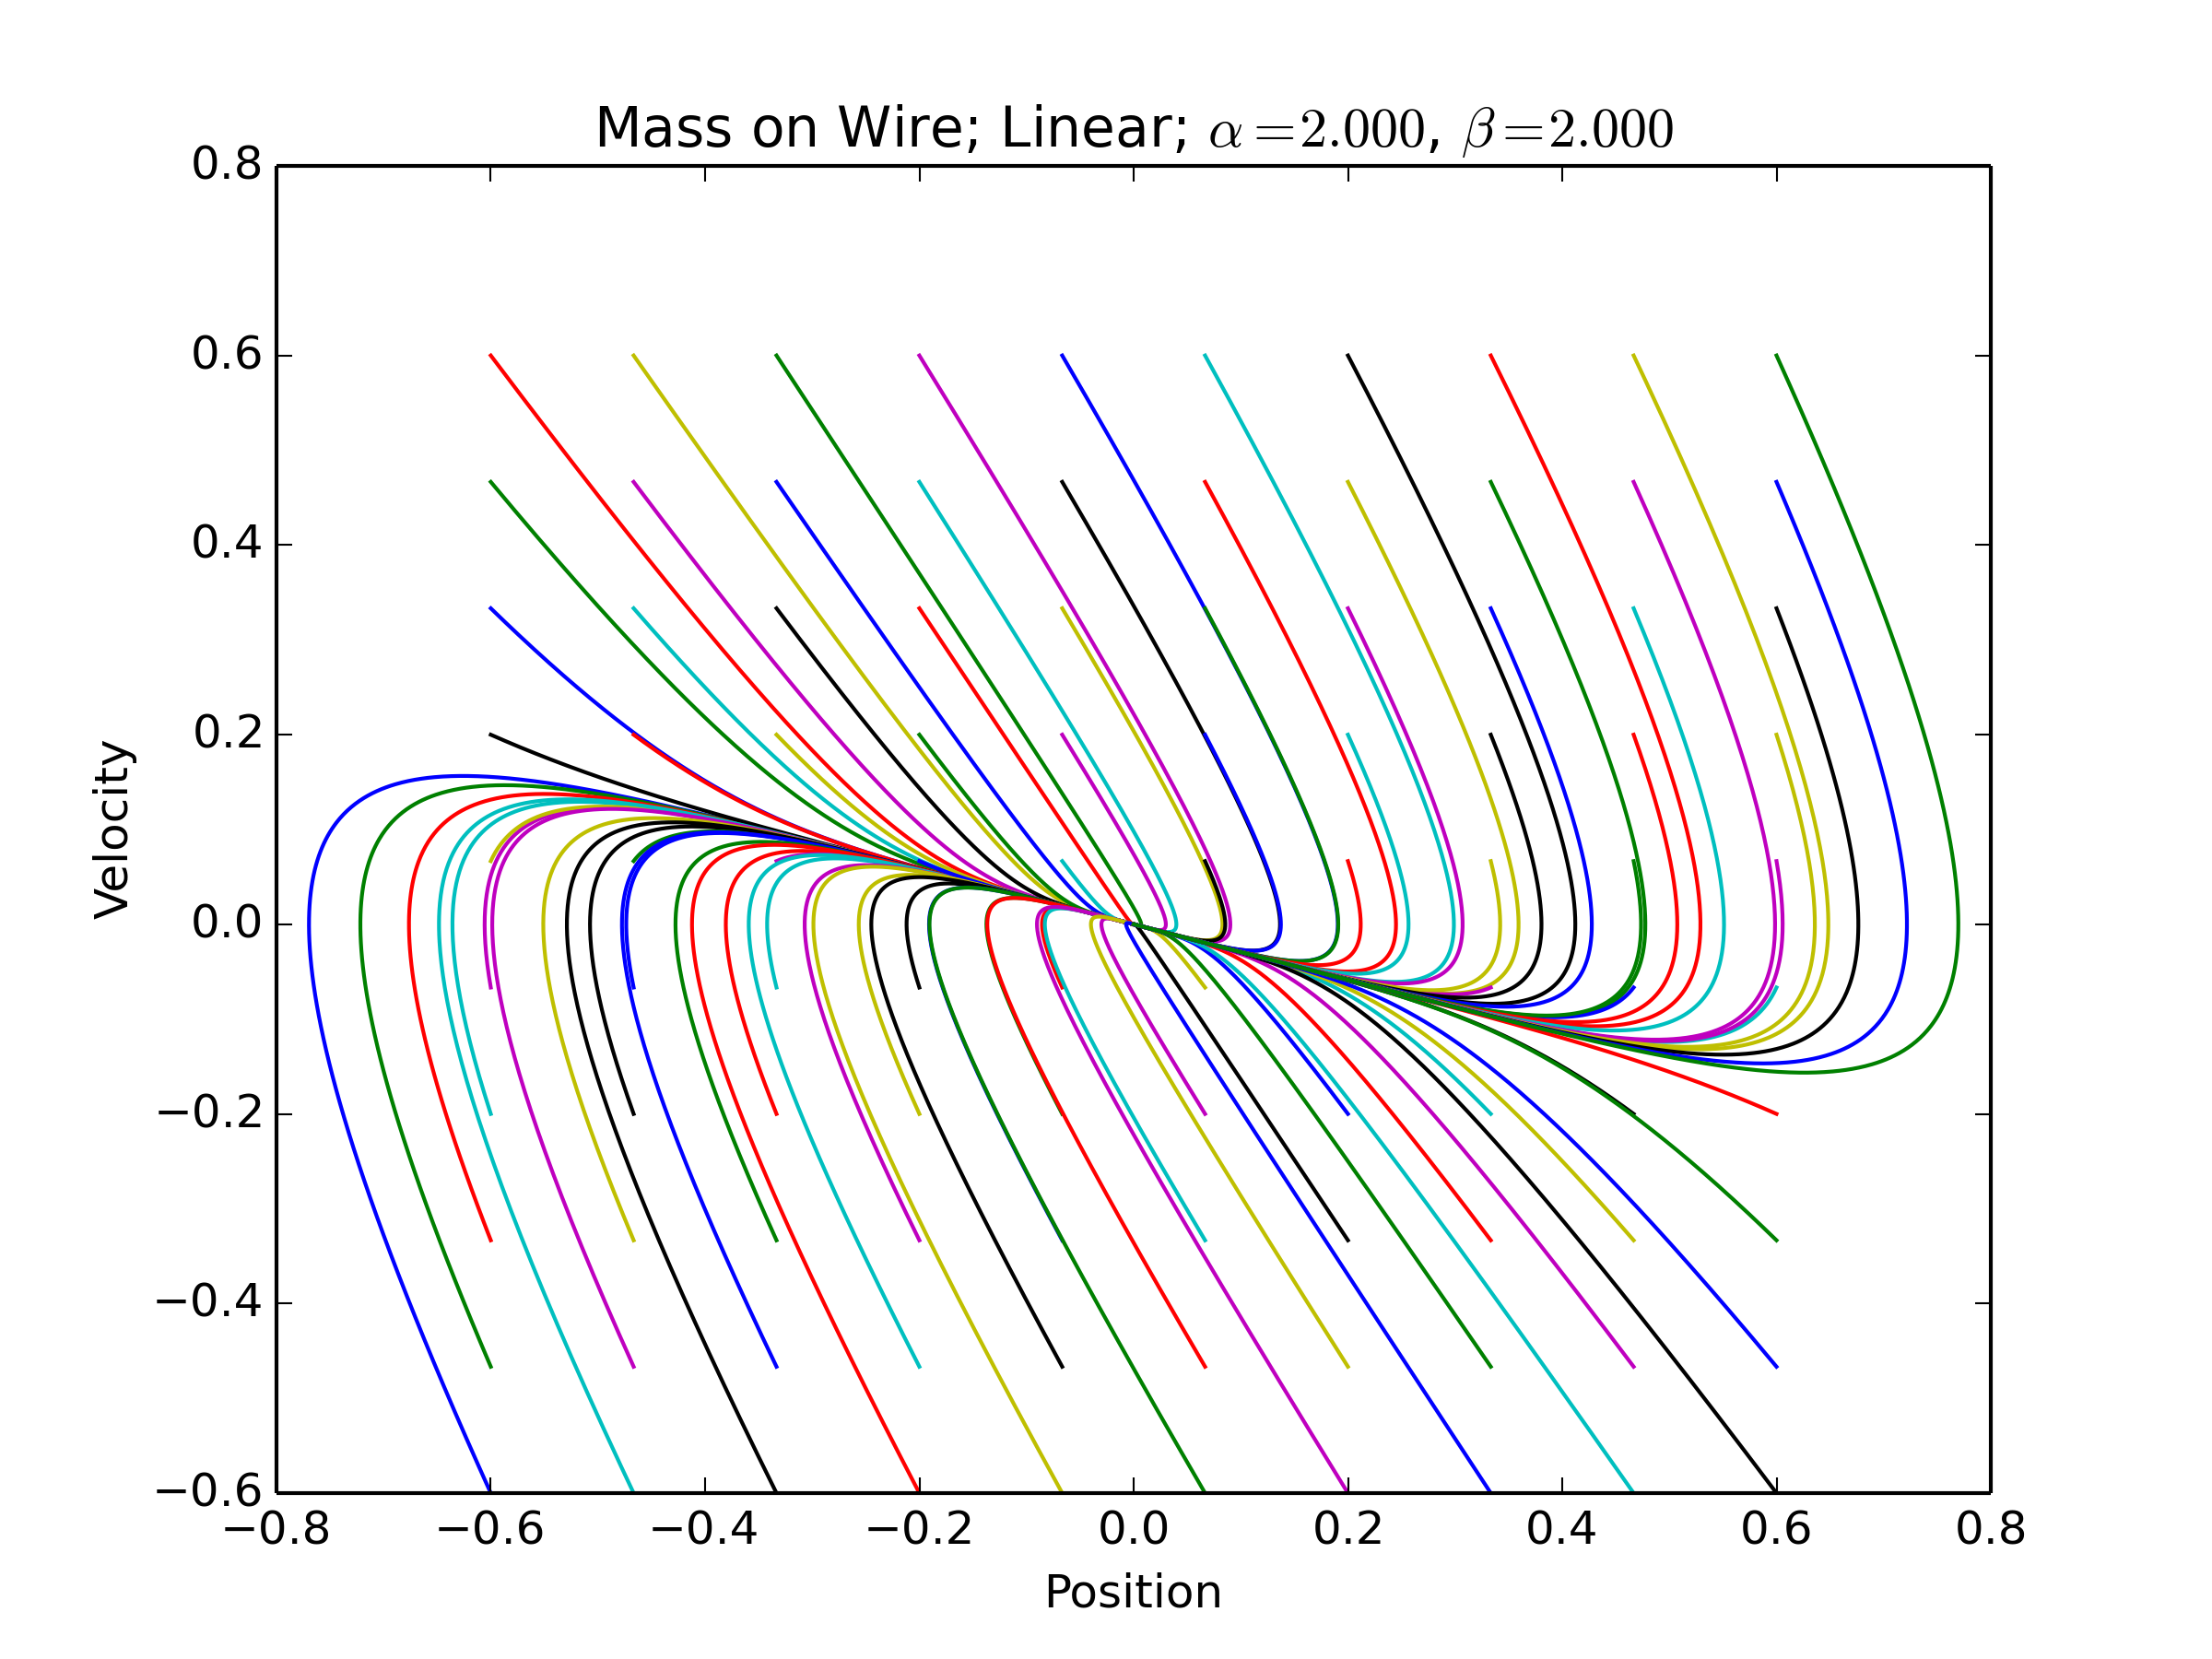
\includegraphics[width=400px]{figures/1_d_Mass_on_Wire_linear}
    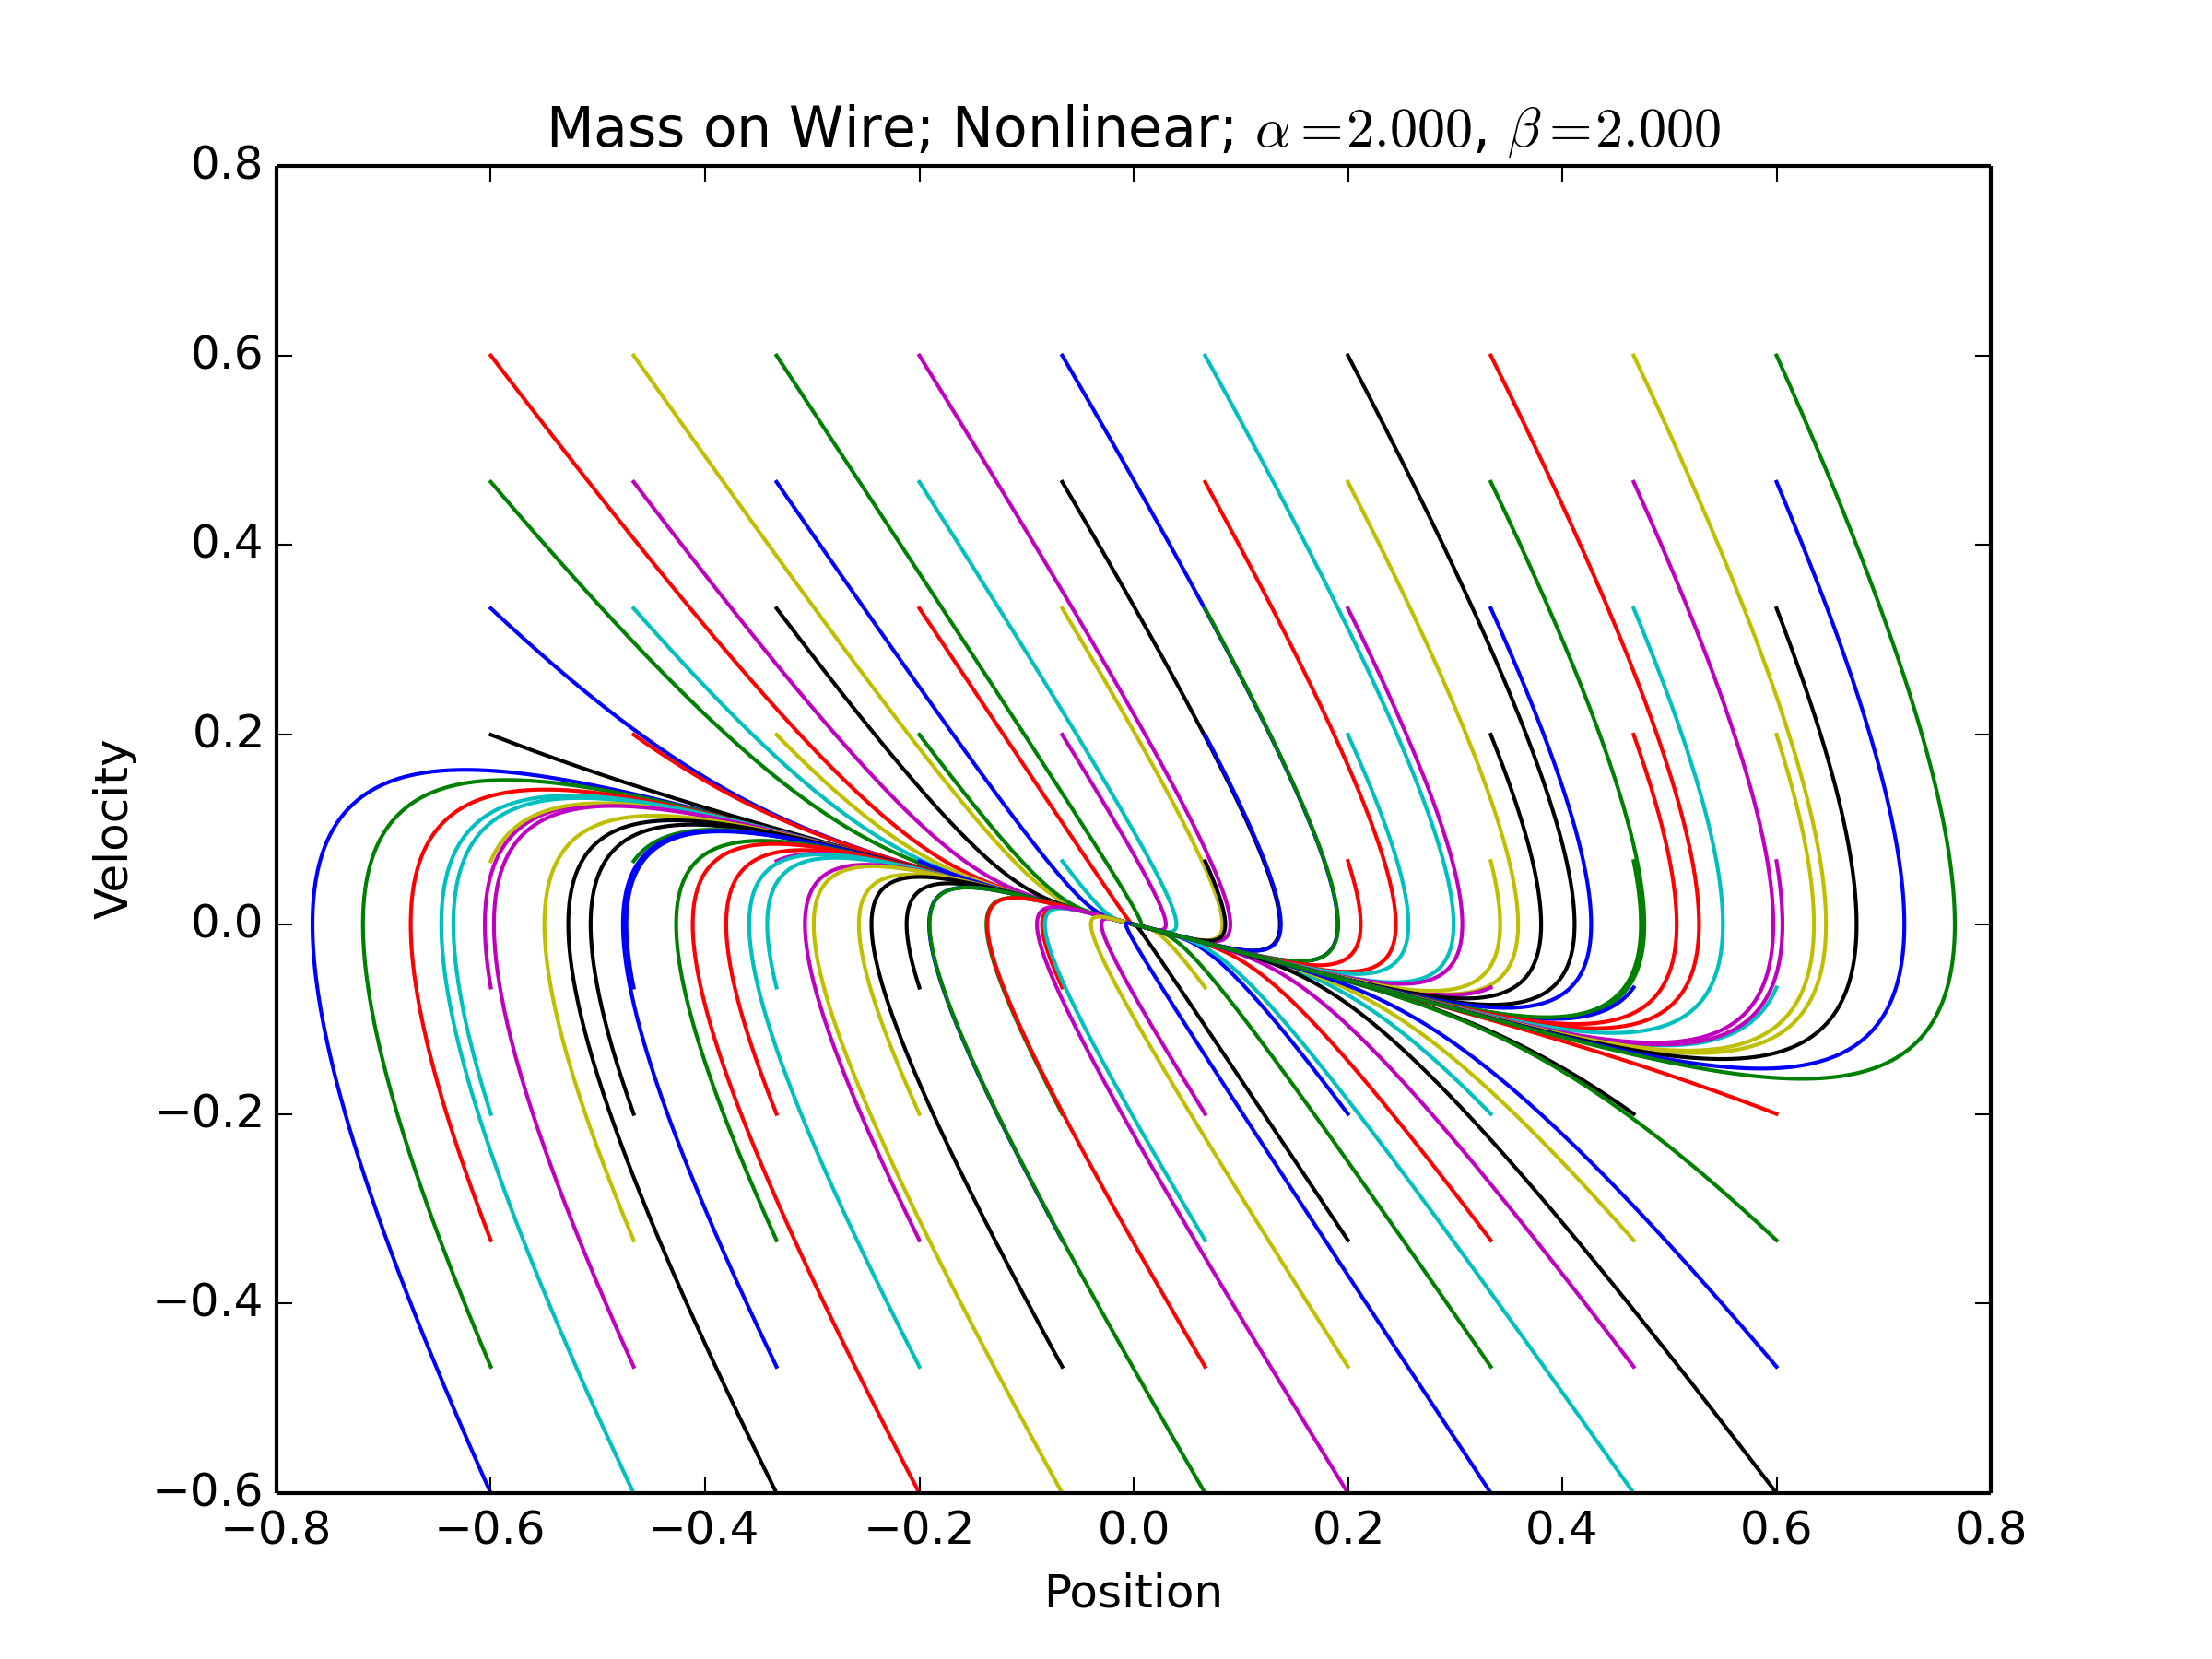
\includegraphics[width=400px]{figures/1_d_Mass_on_Wire_nonlinear}
\end{figure}
\begin{figure}[ht]
    \centering
    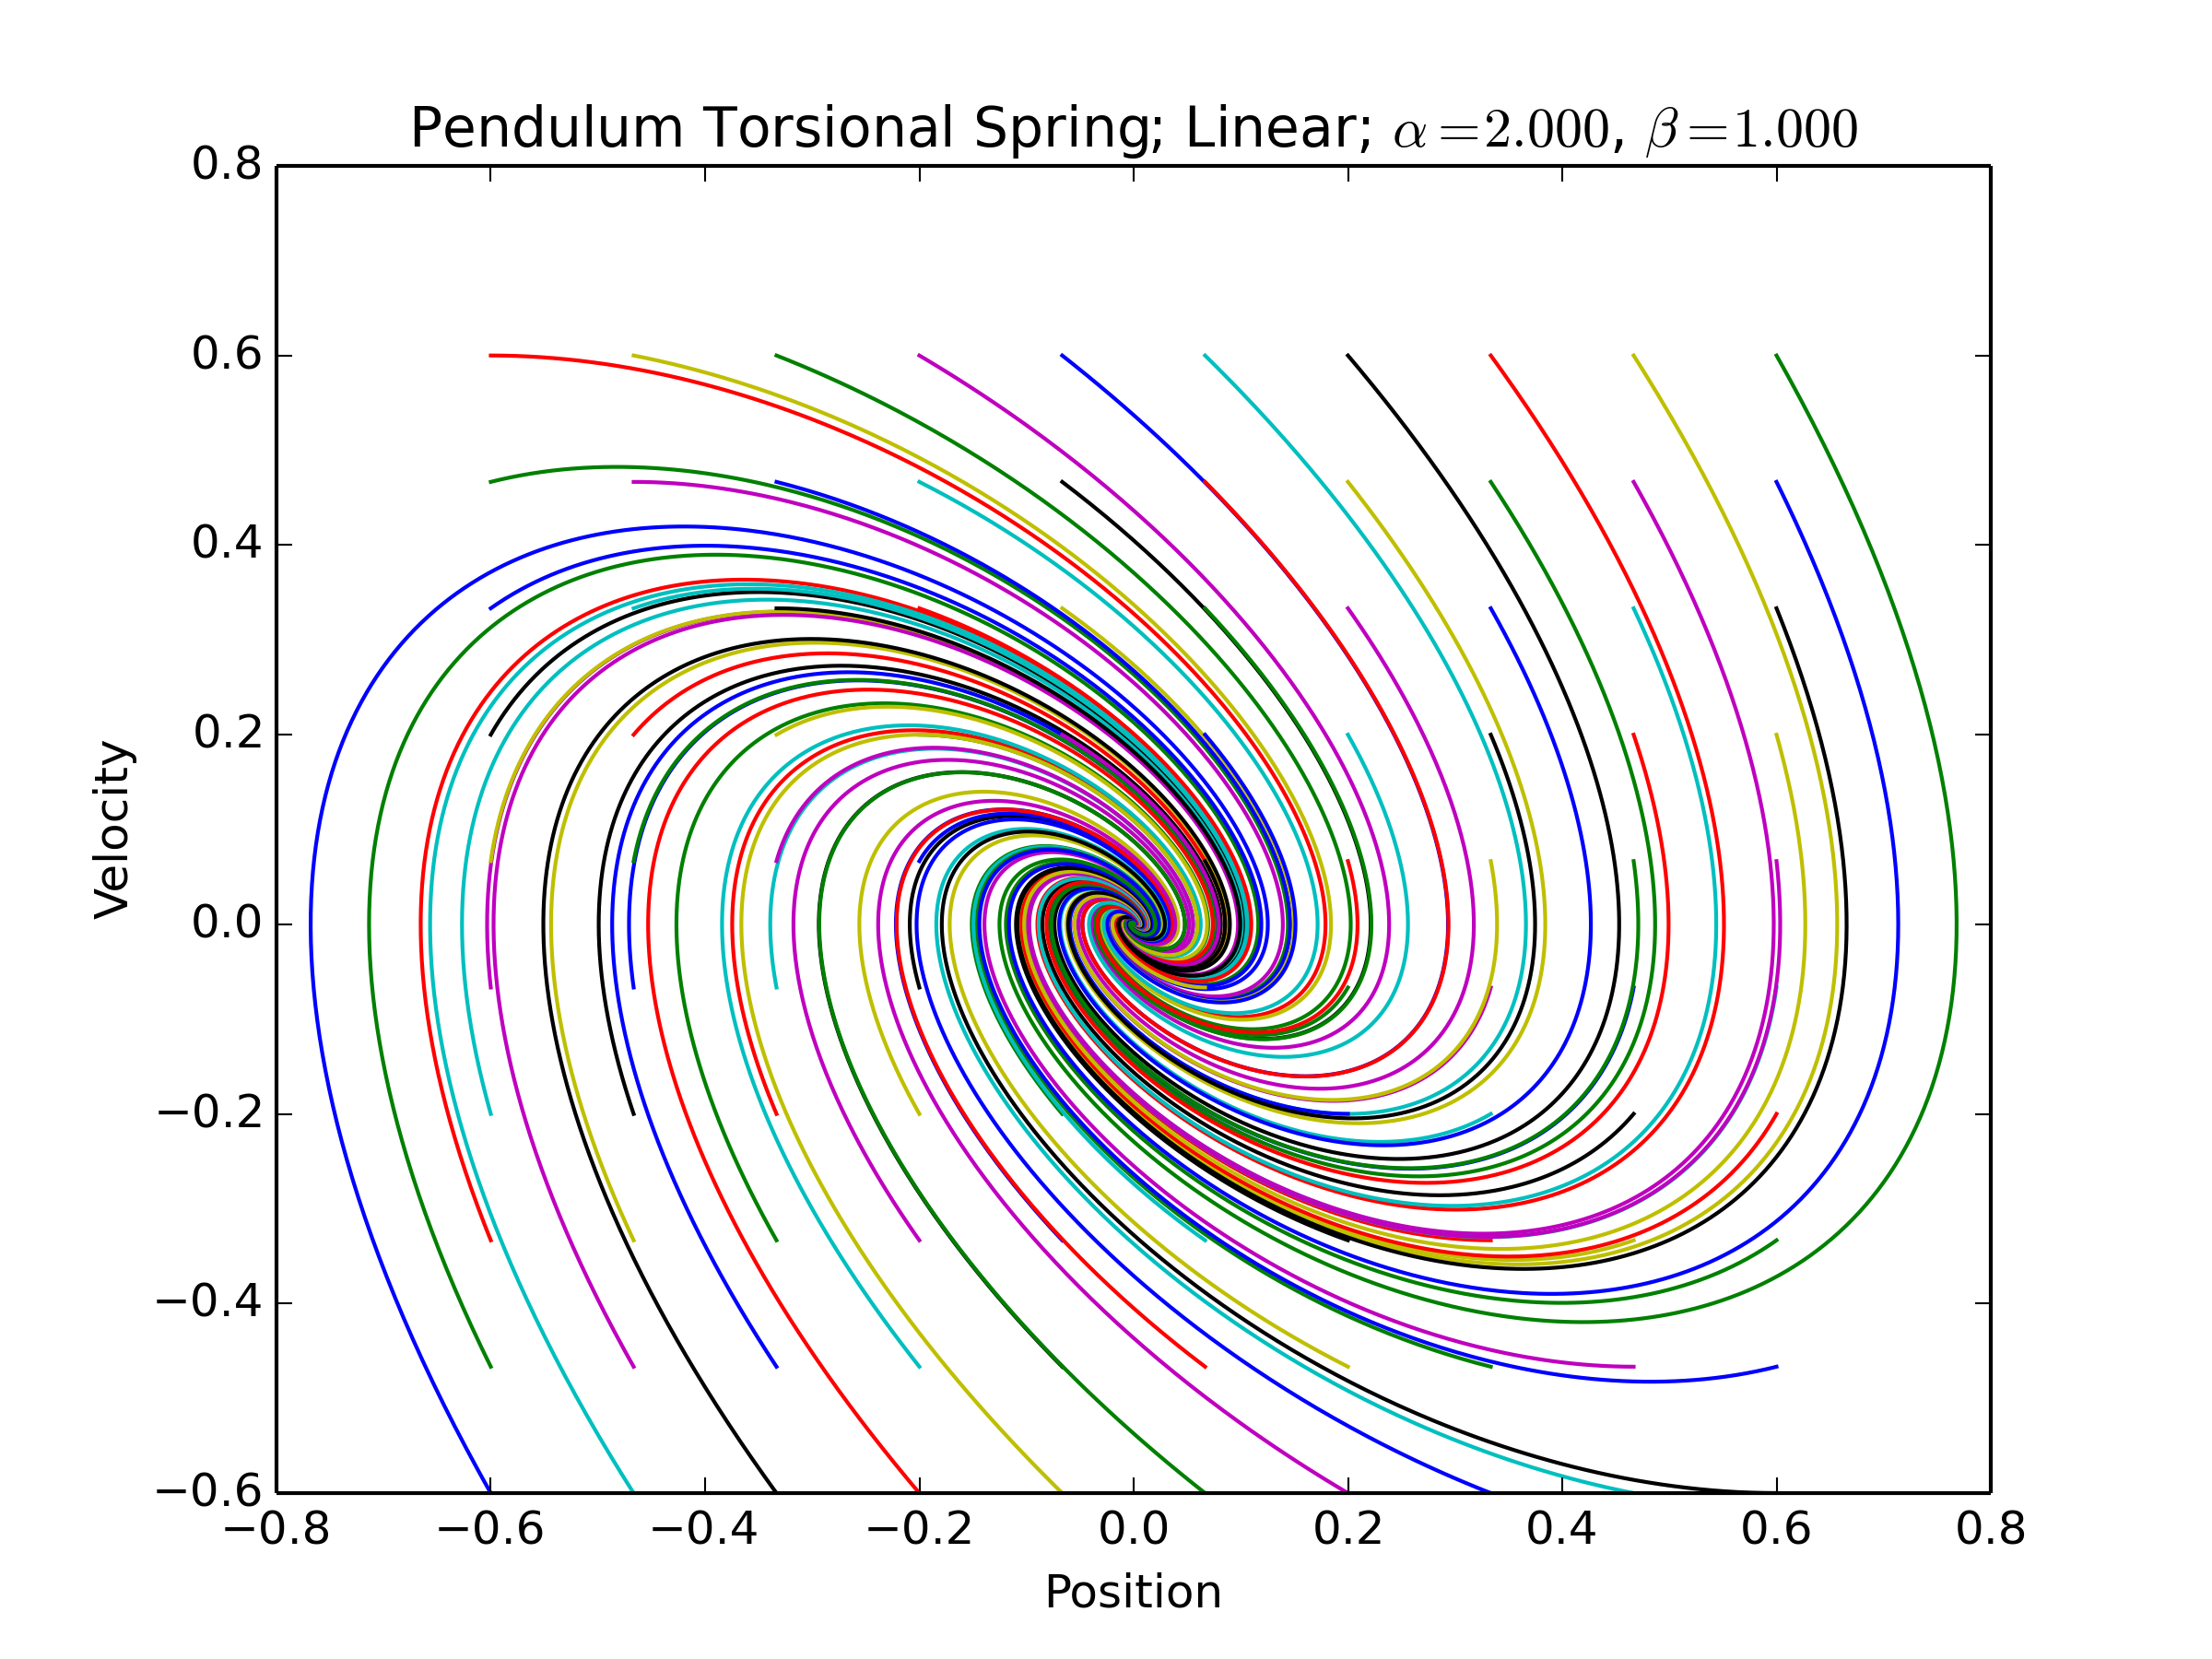
\includegraphics[width=400px]{figures/1_d_Pendulum_Torsional_Spring_linear}
    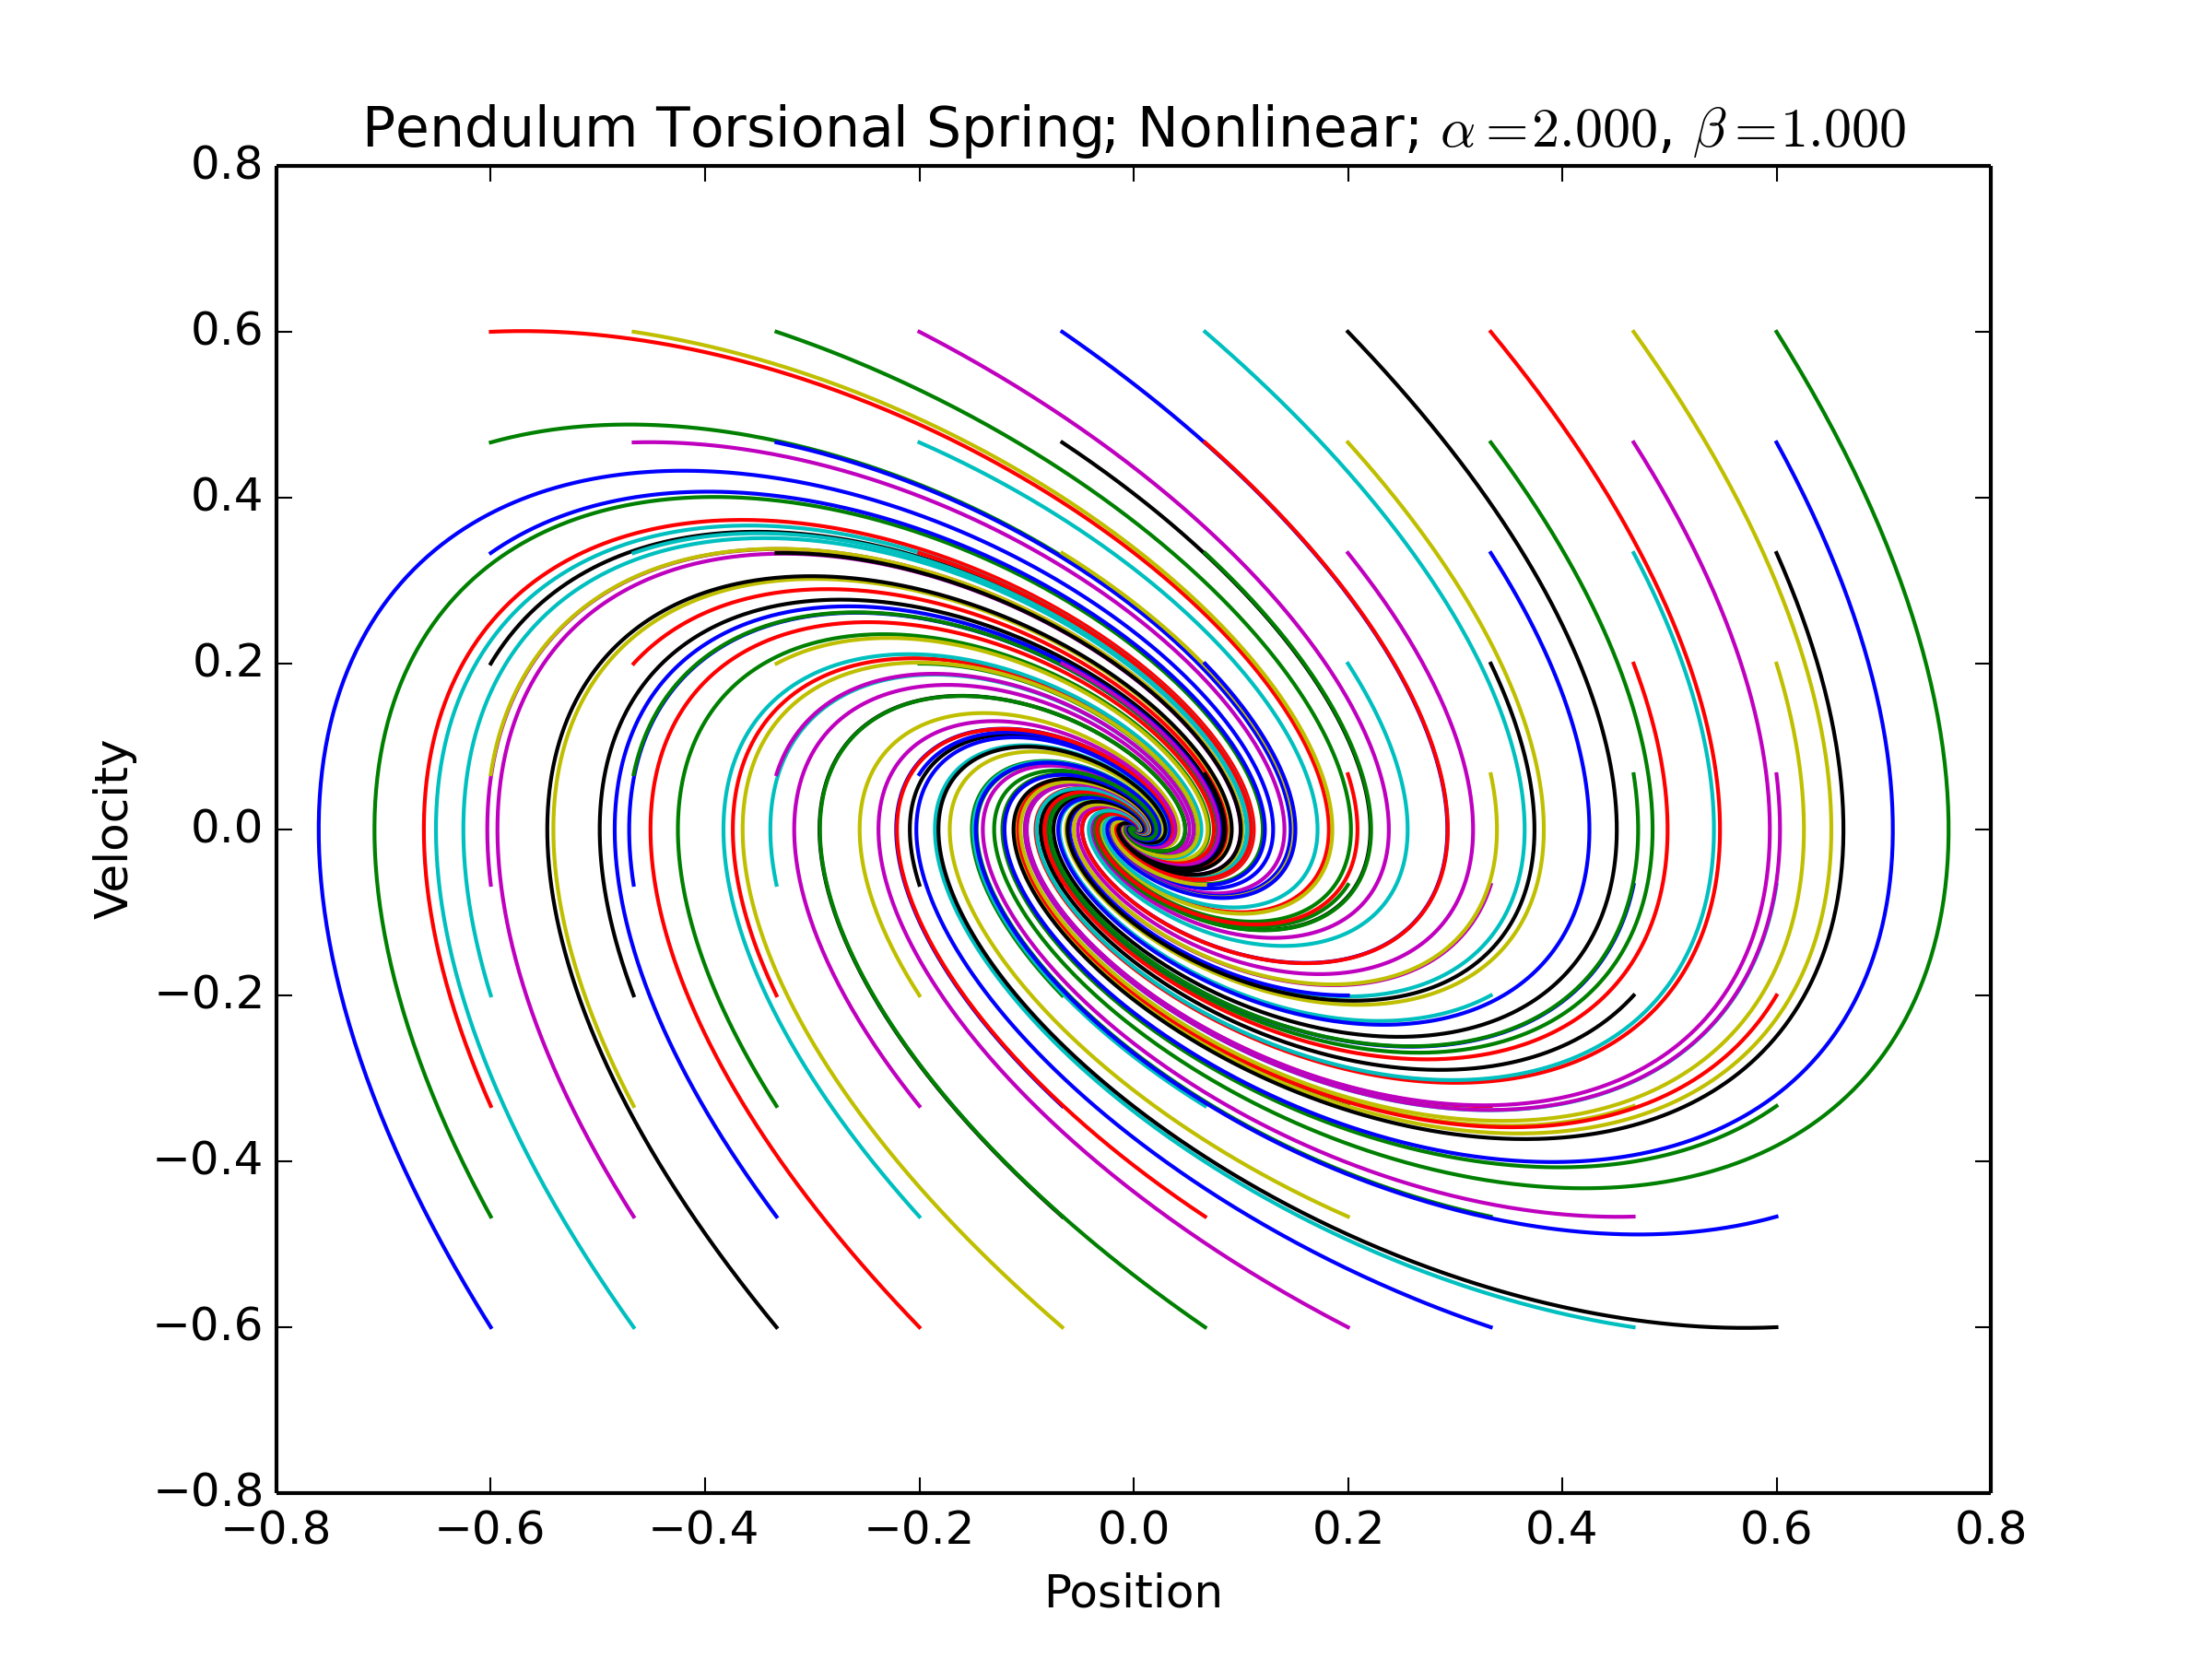
\includegraphics[width=400px]{figures/1_d_Pendulum_Torsional_Spring_nonlinear}
\end{figure}
\begin{figure}[ht]
    \centering
    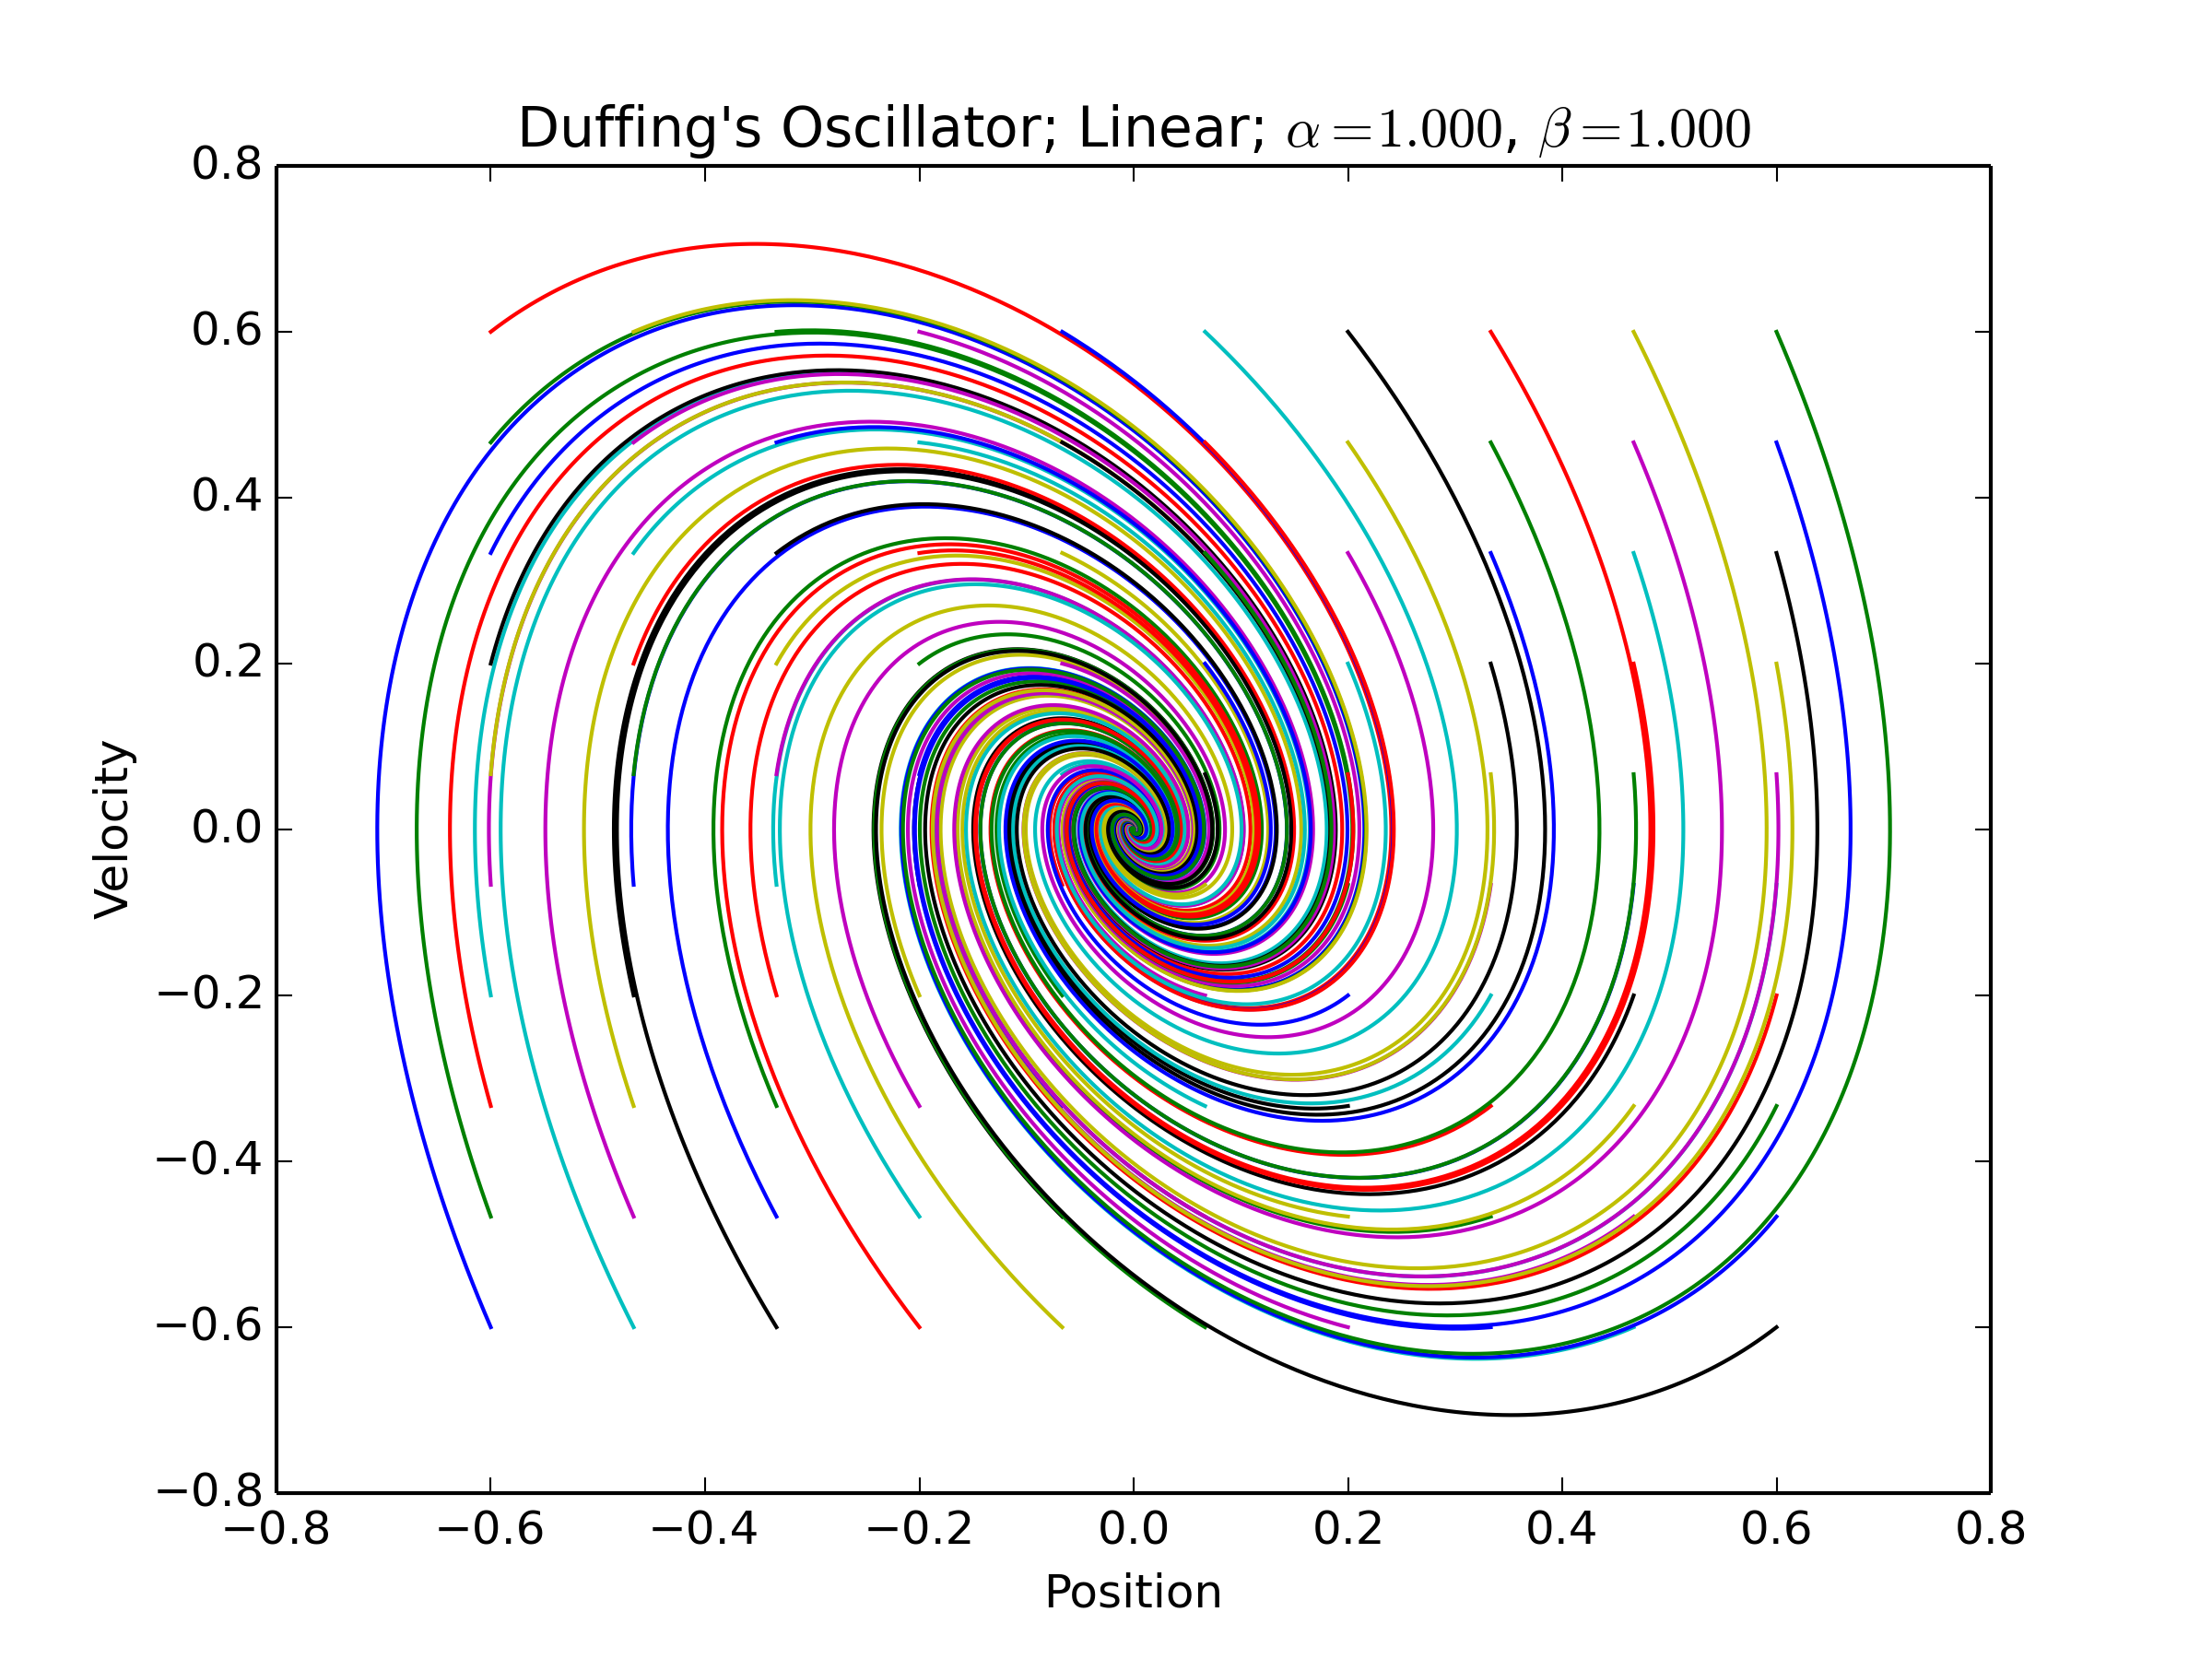
\includegraphics[width=400px]{figures/1_d_Duffing's_Oscillator_linear}
    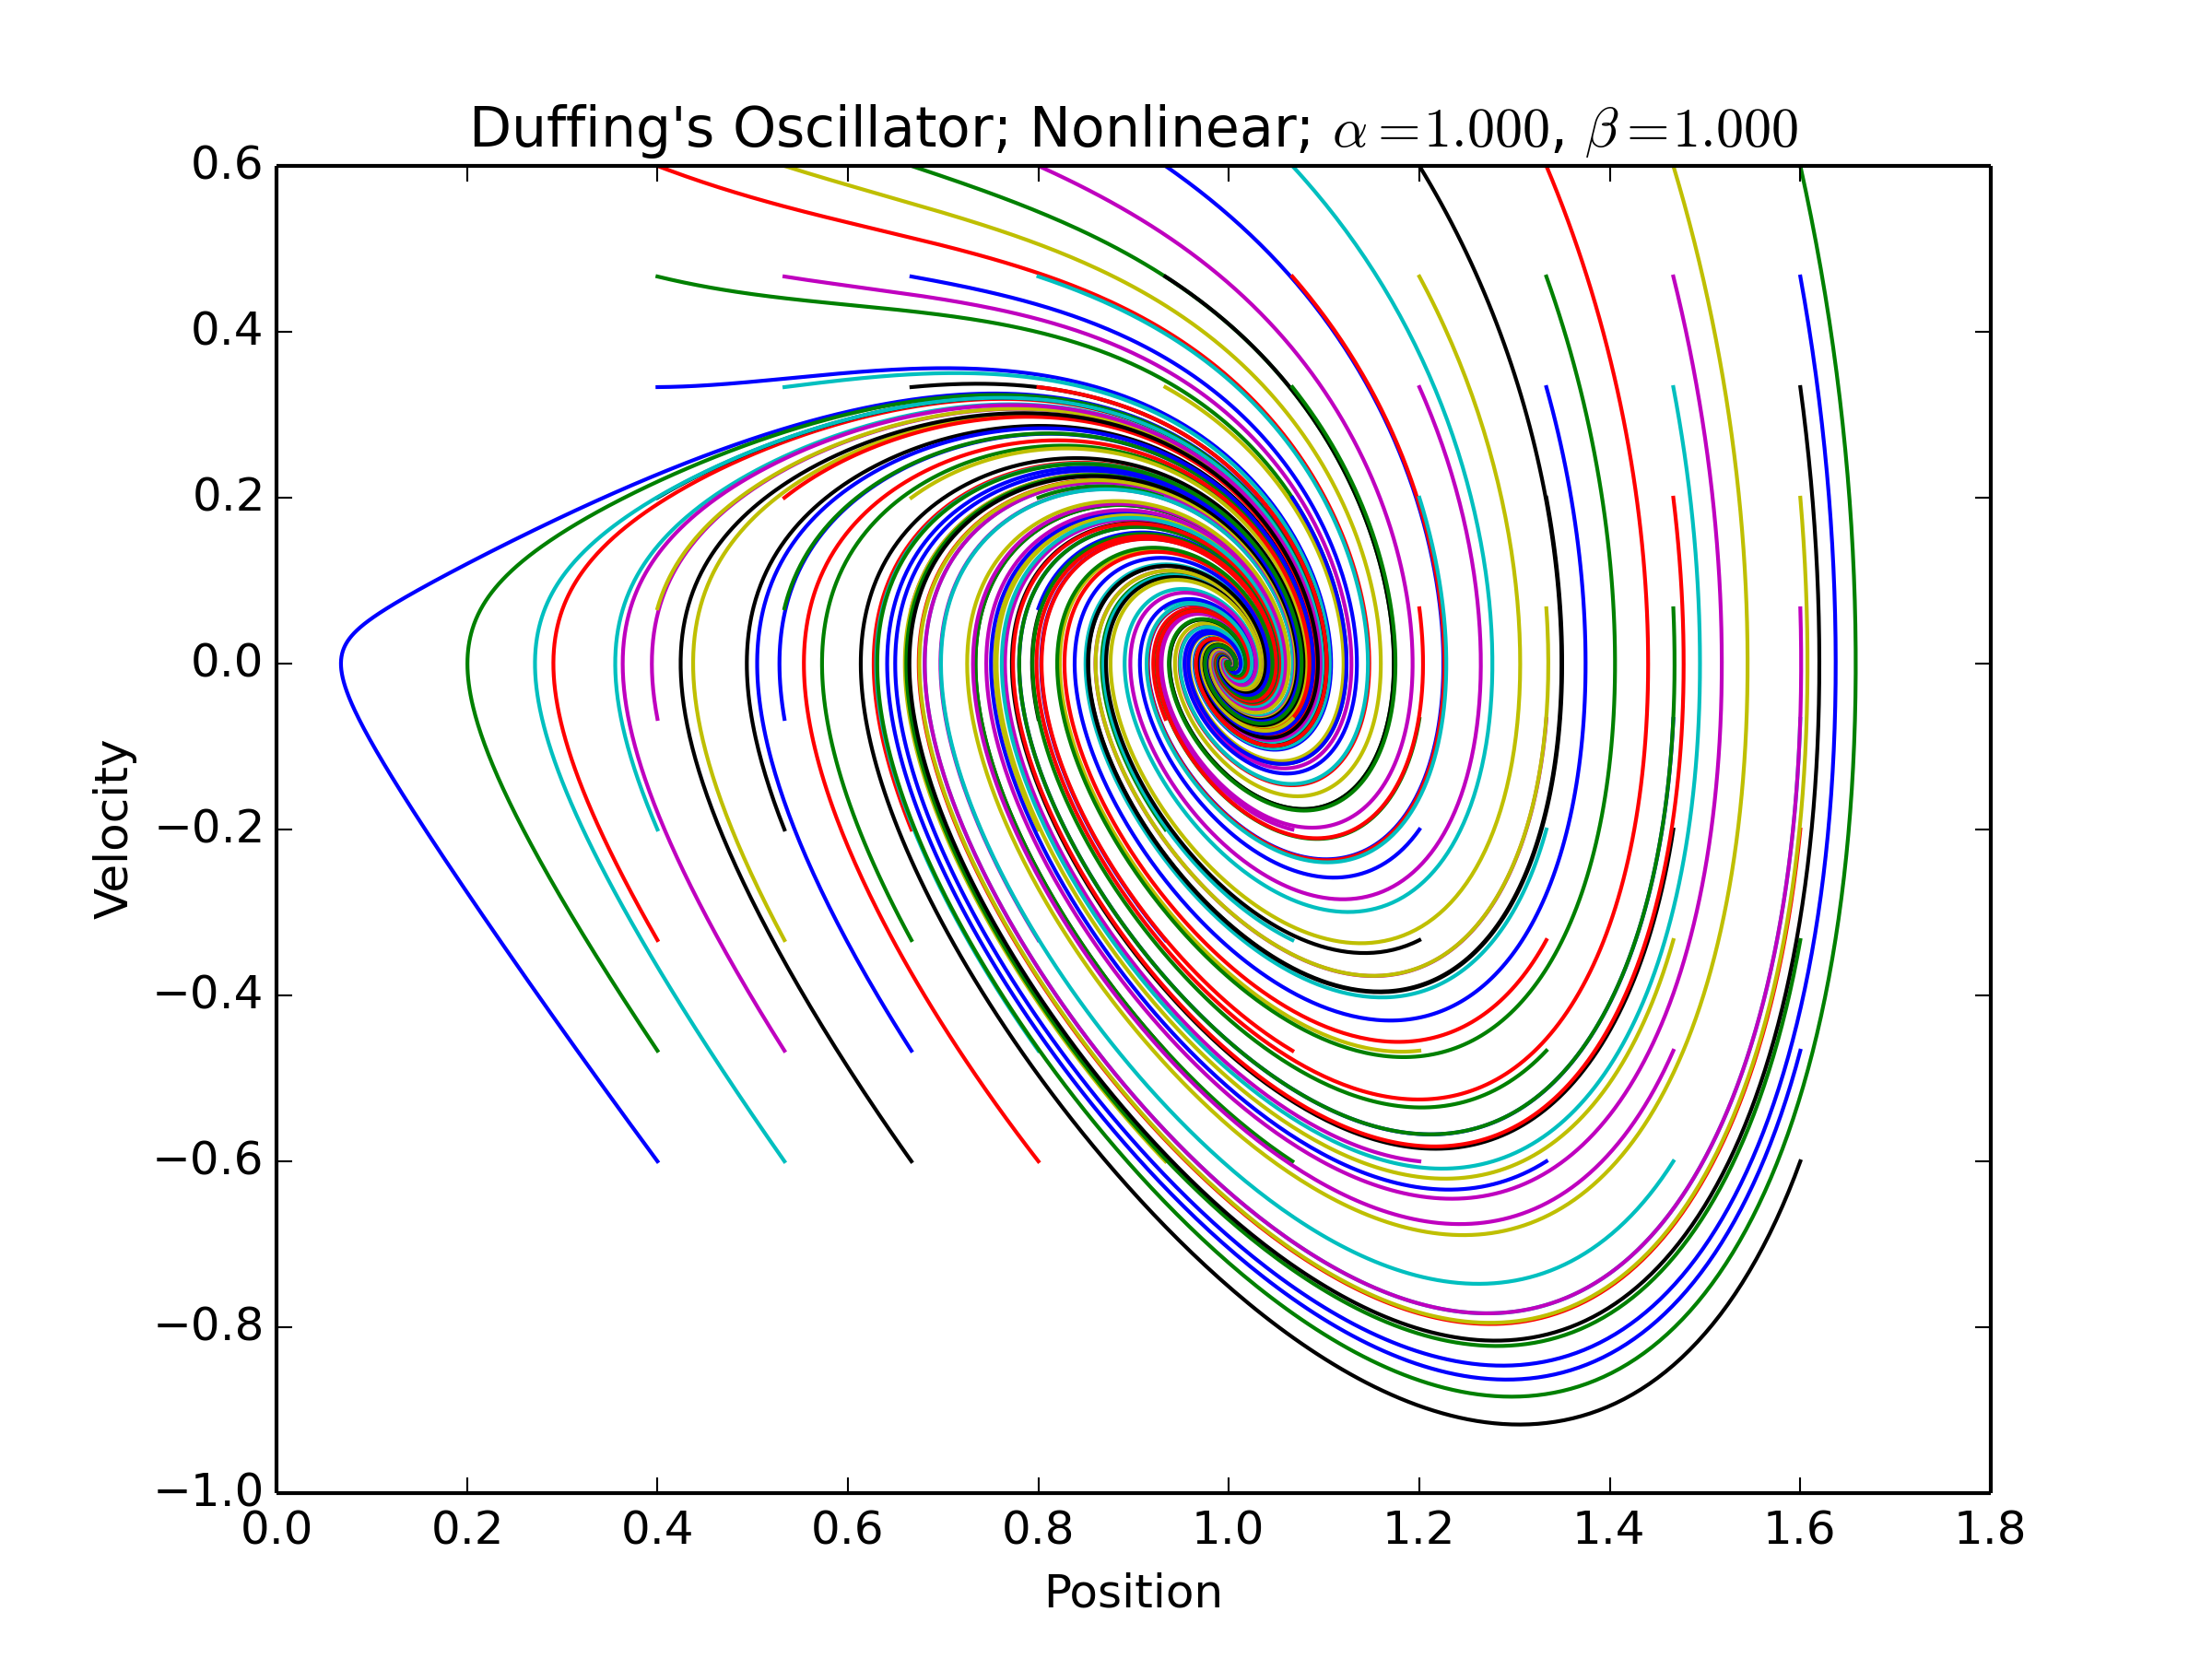
\includegraphics[width=400px]{figures/1_d_Duffing's_Oscillator_nonlinear}
\end{figure}

\FloatBarrier
\section*{Problem 2}
\emph{Problem 6.3.3}

\subsection*{ a)}
\emph{Find all fixed points, classify them and fill in the rest of your phase portrait for the following system of equations.}
\begin{align*}
	\dot{x} &= 1 + y - e^{-x} \\
	\dot{y} &= x^3 - y
\end{align*}

To solve for equilibrium points, set $\dot{x} = \dot{y} = 0$.  Then solve both for $y$ to yield
\begin{align*}
	y &= e^{-x} - 1 \\
	y &= x^3
\end{align*}
Since $e^{-x} - 1$ is a strictly decreasing function of $x$, and $x^3$ is a strictly increasing function of $x$, this system has at most one solution.  Since $(x,y) = (0,0)$ is a solution, it must be the only solution.  Thus $\vec{x}^* = [0,0]^T$ is the only fixed point.  The Jacobian is
\begin{align*}
	J &= \qty(\begin{array}{cc}
		e^{-x} & 1 \\
		3x^2 & -1
	\end{array}) \\
	\implies J_{\vec{x}^*} &= \qty(\begin{array}{cc}
		1 & 1 \\
		0 & -1
	\end{array})
\end{align*}
which is a triangular matrix, and so the eigenvalues are $\lambda_{1,2} = \pm 1$, which shows $\vec{x}^*$ is a saddle.

\subsection*{ b)}
\emph{Check your answers by generating a phase portrait with Matlab.  (Simulate several initial conditions, and plot $x$ and $y$)}

\begin{figure}[ht]
    \centering
    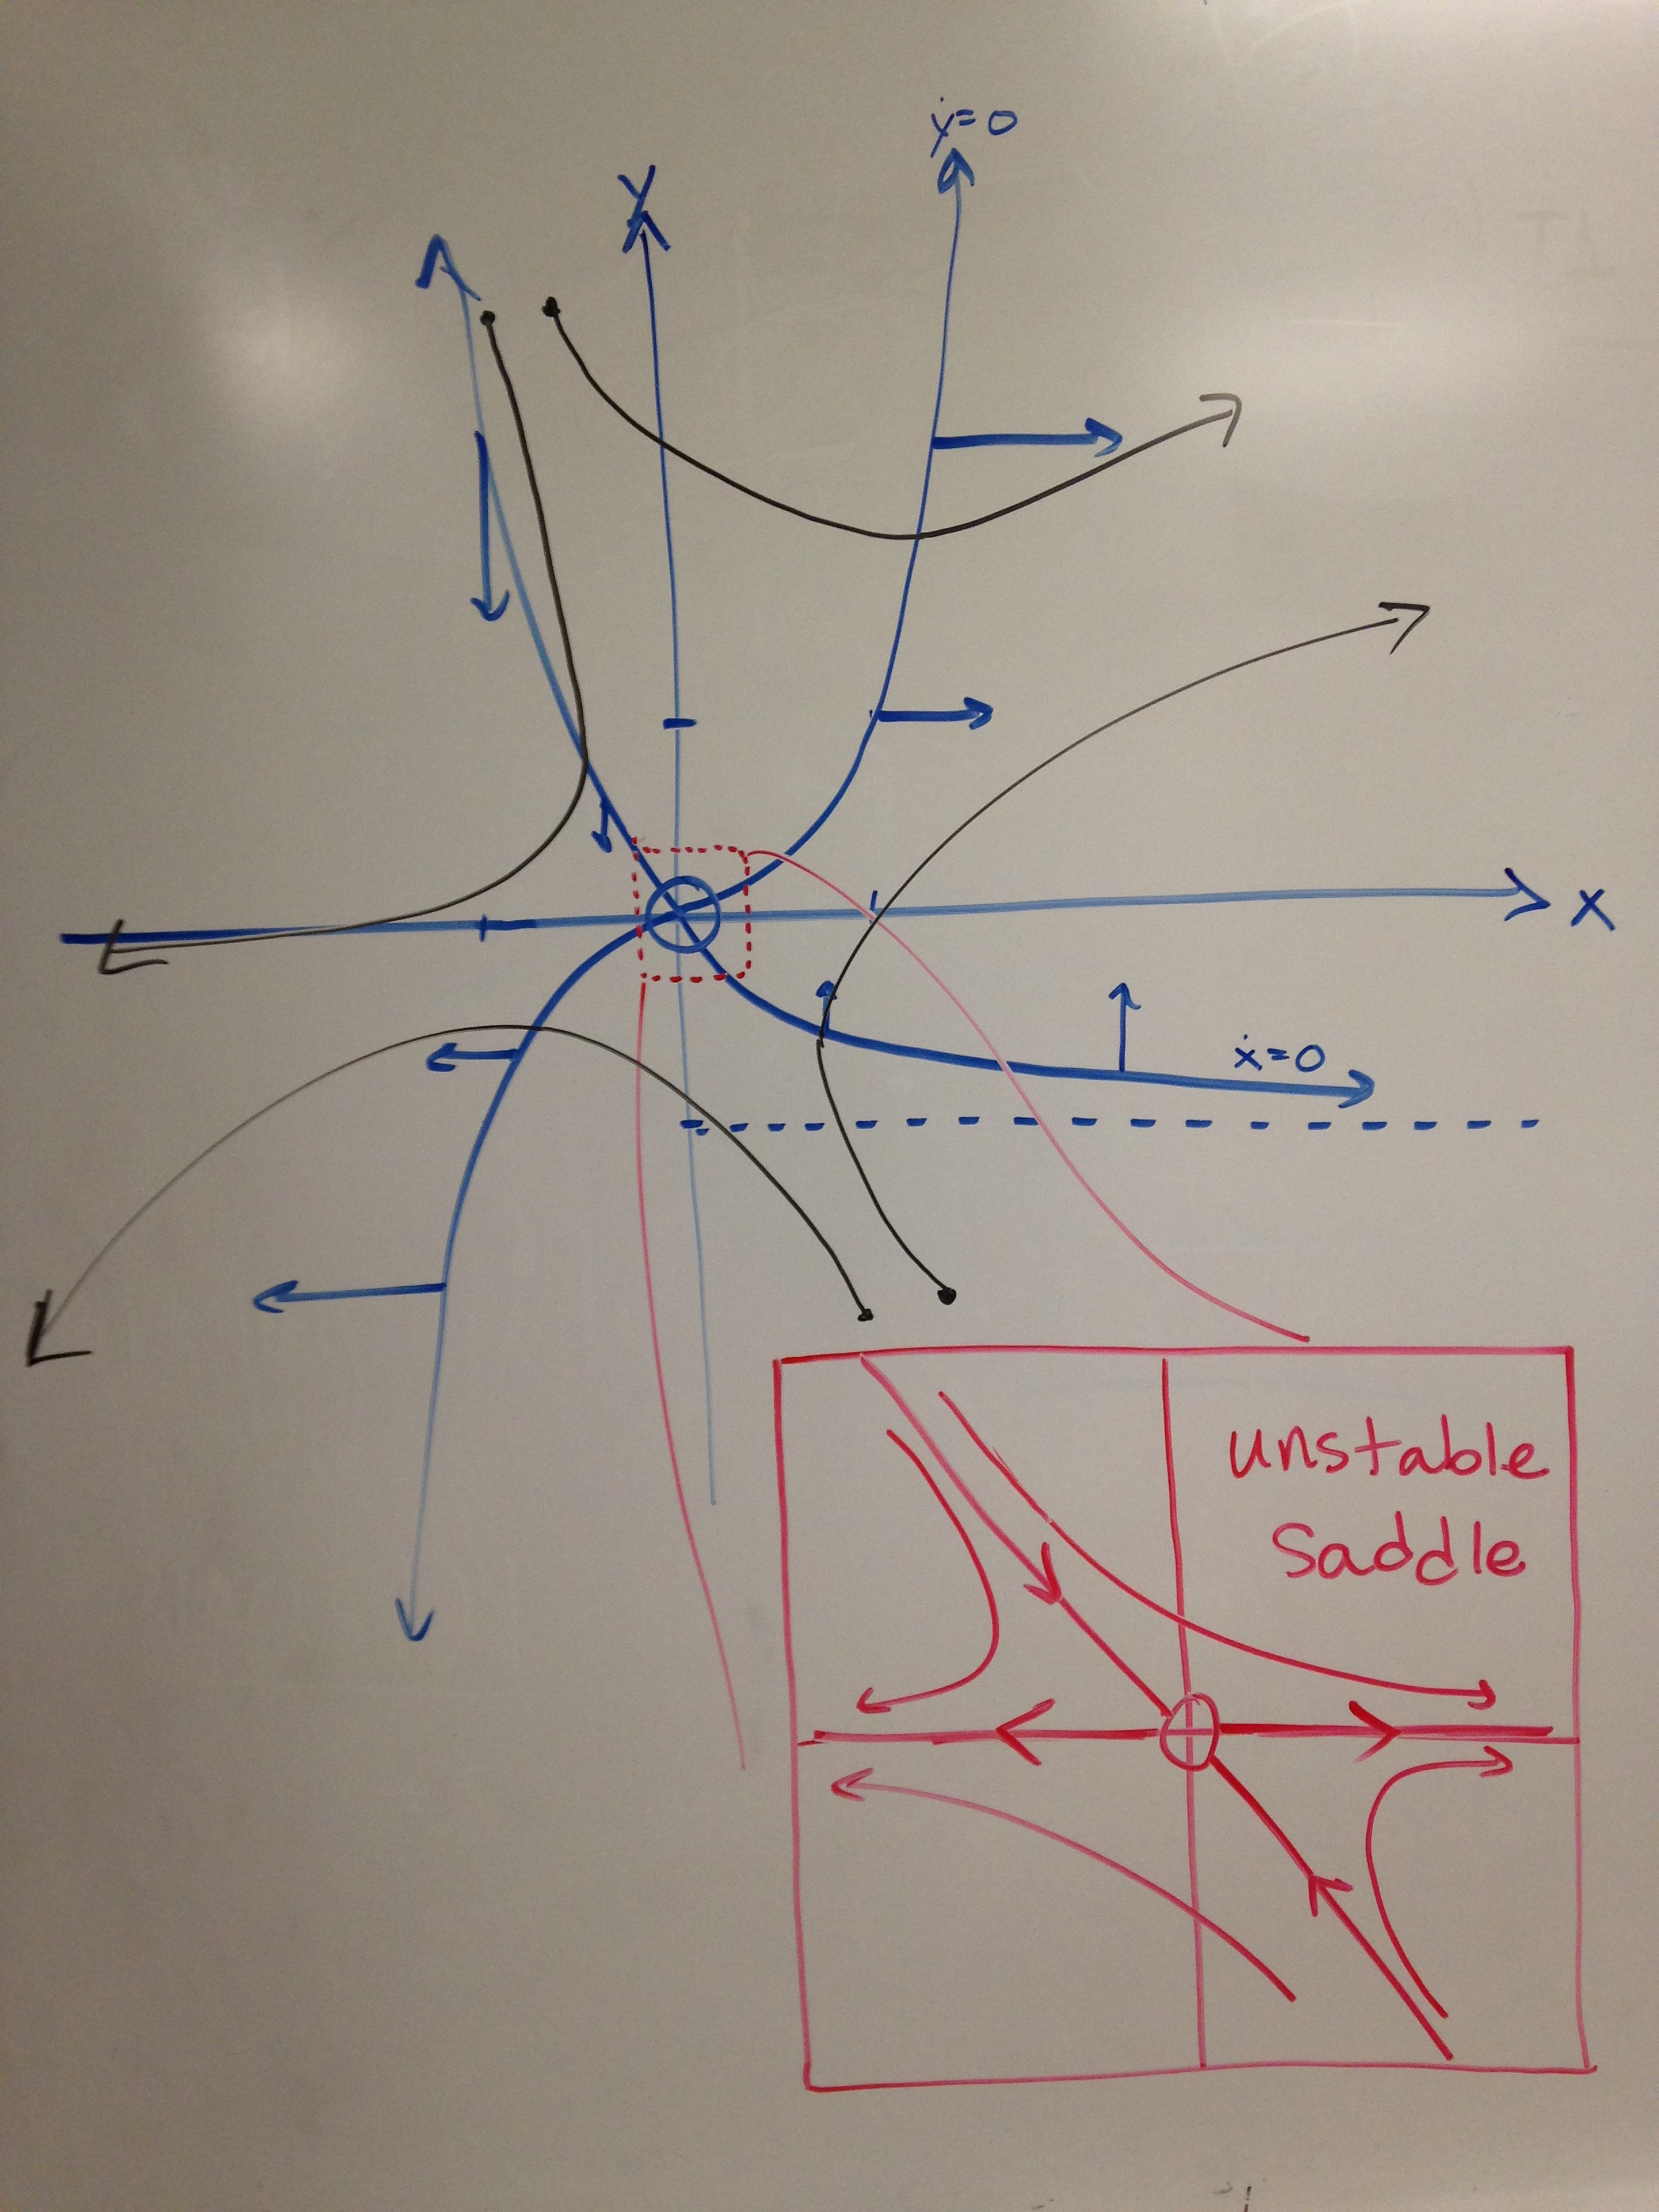
\includegraphics[height=350px]{figures/2_drawing.jpg}
    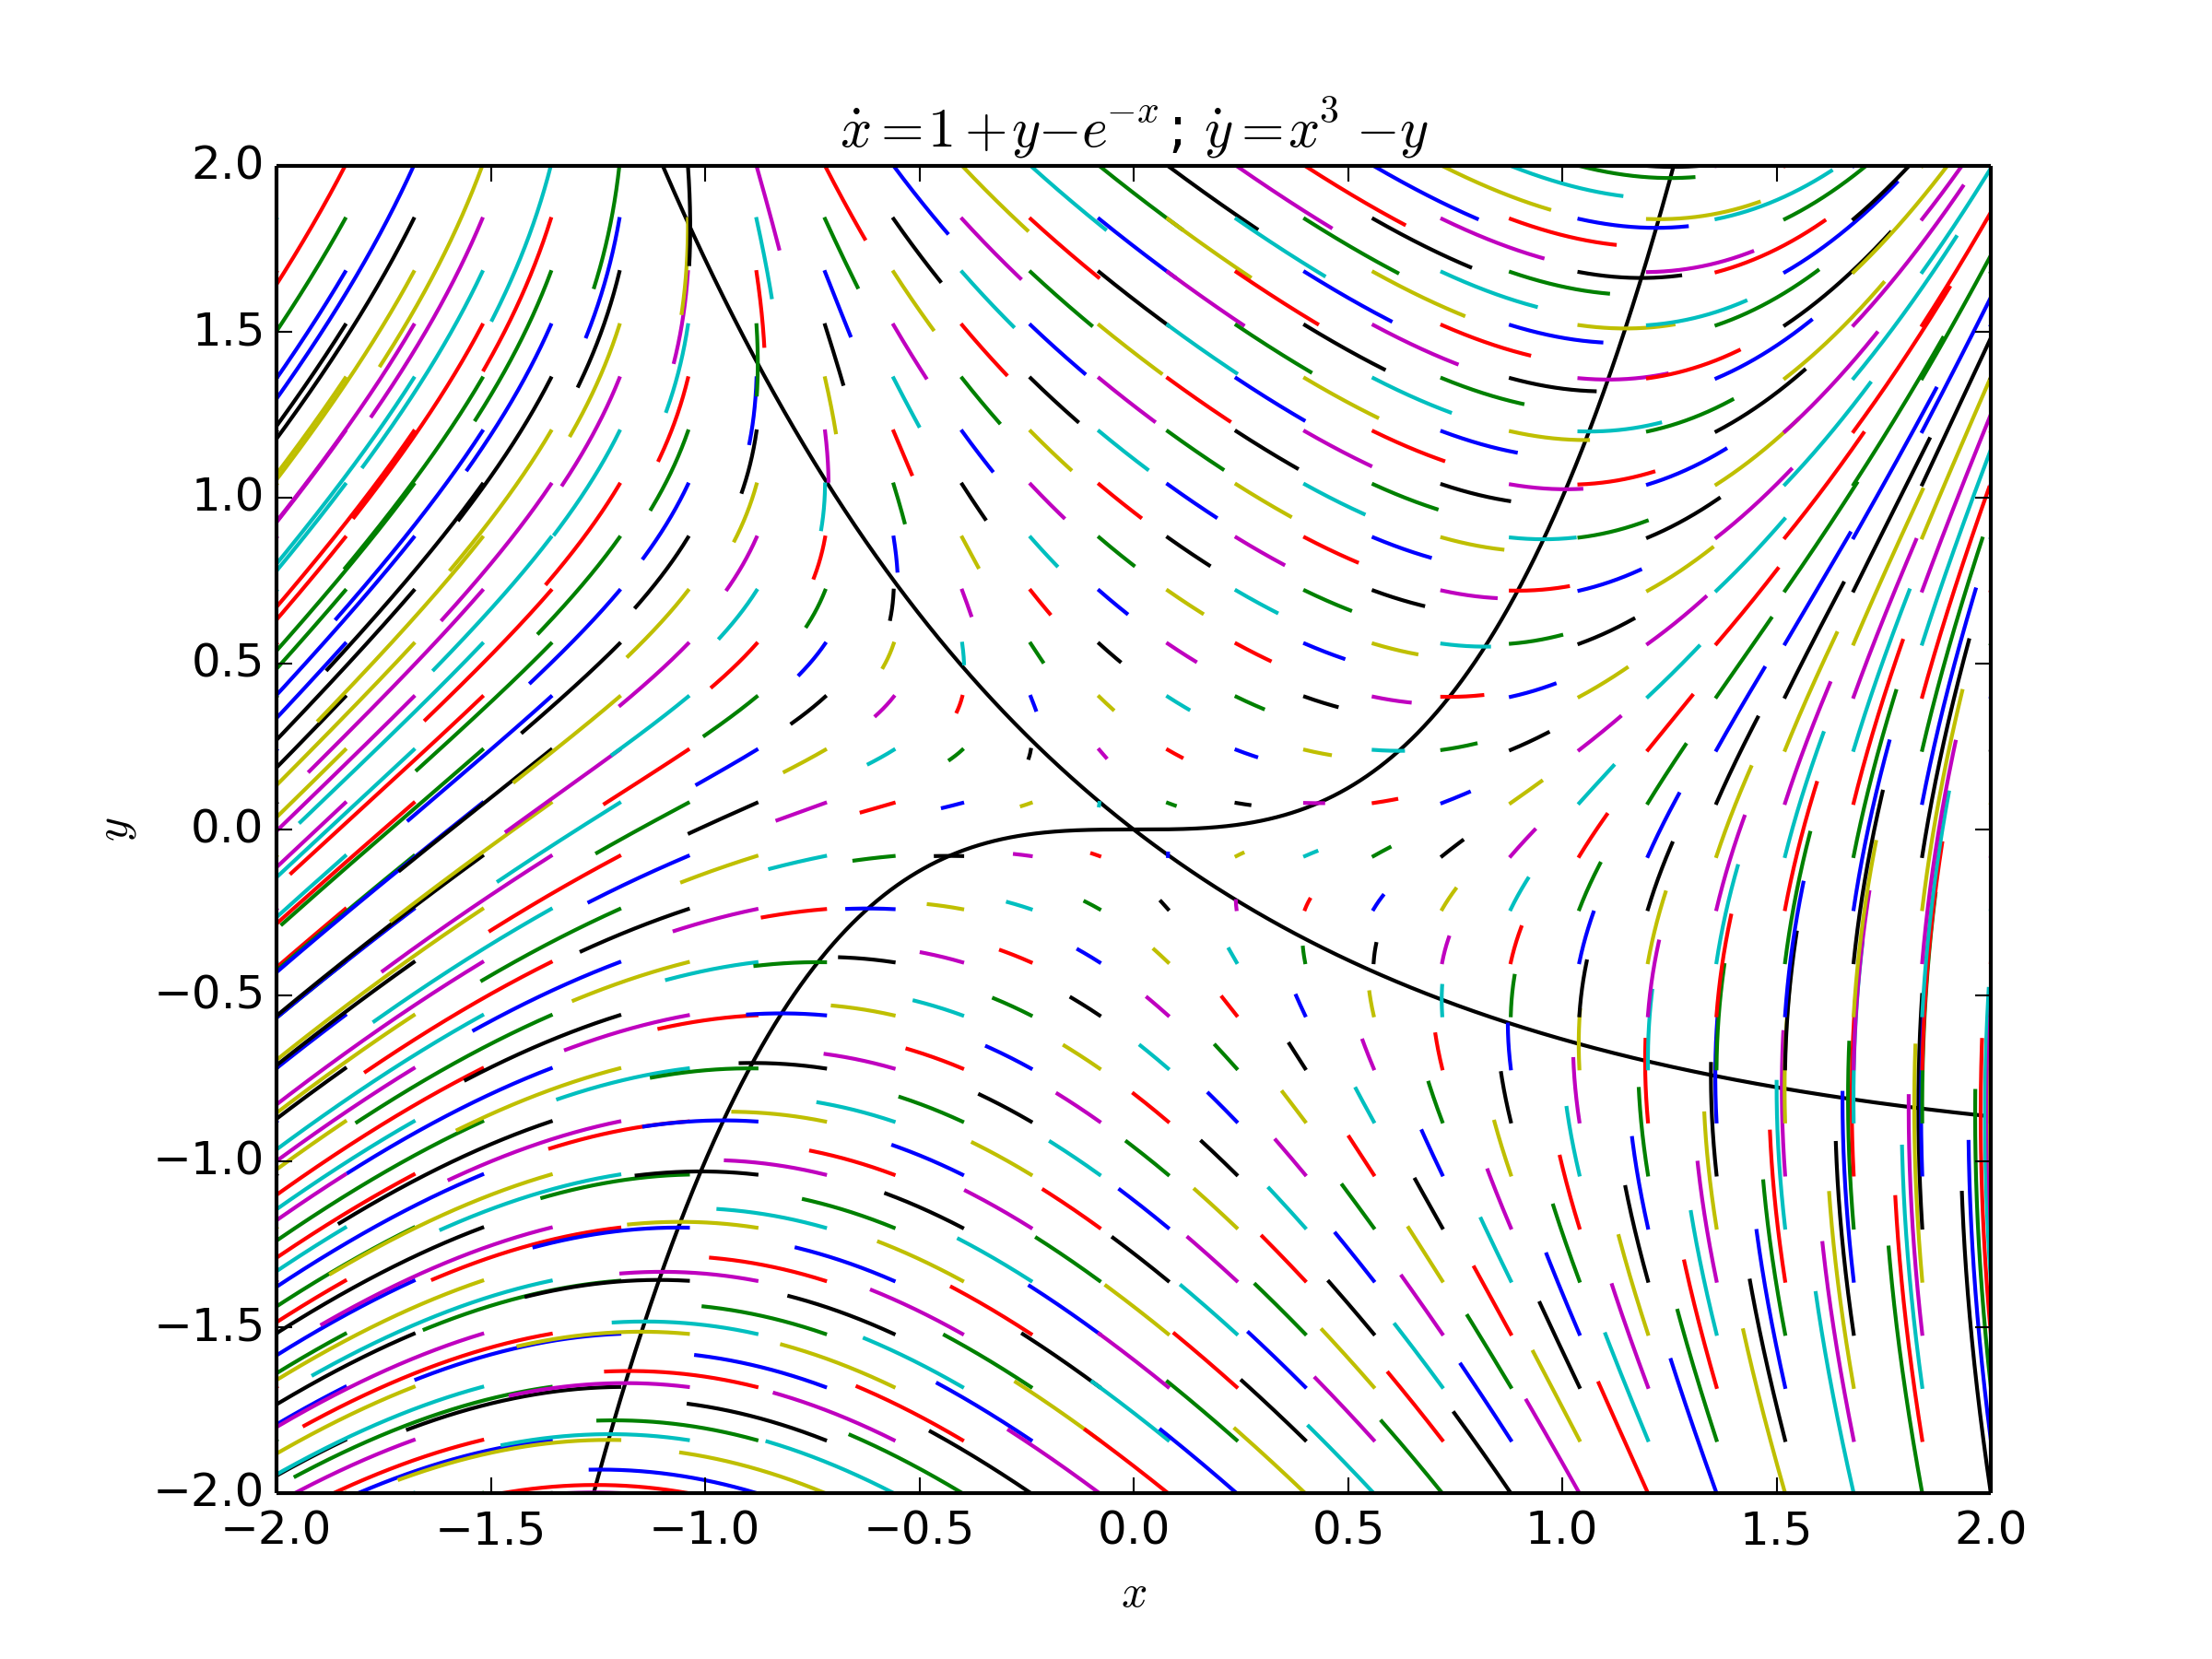
\includegraphics[width=400px]{figures/2_simulation.png}
\end{figure}

\FloatBarrier
\section*{Problem 3}
\emph{Problem 6.3.6}

\subsection*{ a)}
\emph{Find all fixed points, classify them and fill in the rest of your phase portrait for the following system of equations.}
\begin{align*}
	\dot{x} &= xy - 1 \\
	\dot{y} &= x - y^3
\end{align*}
Set $\dot{x} = \dot{y} = 0$, and substitute $x = y^3$ in to $\dot{x} = 0$, yielding $y^4 = 1$, i.e. $y = \pm 1$.  $y = 1 \implies x = 1$, and $y = -1 \implies x = -1$.  Thus the fixed points are $\vec{x_A}^* = [1,1]^T$ and $\vec{x_B}^* = [-1,-1]^T$.  The Jacobian is
\begin{align*}
	J &= \qty(\begin{array}{cc}
		y & x \\
		1 & -3y^2
	\end{array}) \\
	\implies J_{\vec{x_A}^*} &= \qty(\begin{array}{cc}
		1 & 1 \\
		1 & -3
	\end{array})\ \ \ \text{and}\ \ \ J_{\vec{x_B}^*} = \qty(\begin{array}{cc}
		-1 & -1 \\
		1 & -3
	\end{array})
\end{align*}
Thus the eigenvalues for $\vec{x_A}^*$ are $\lambda_{1,2} = -1 \pm \sqrt{5}$, and the eigenvalues for $\vec{x_B}^*$ are $\lambda_{1,2} = -2$, which shows $\vec{x_A}^*$ is a saddle and $\vec{x_B}^*$ is a stable node.

\subsection*{ b)}
\emph{Check your answers by generating a phase portrait with Matlab.  (Simulate several initial conditions, and plot $x$ and $y$)}

\begin{figure}[ht]
    \centering
    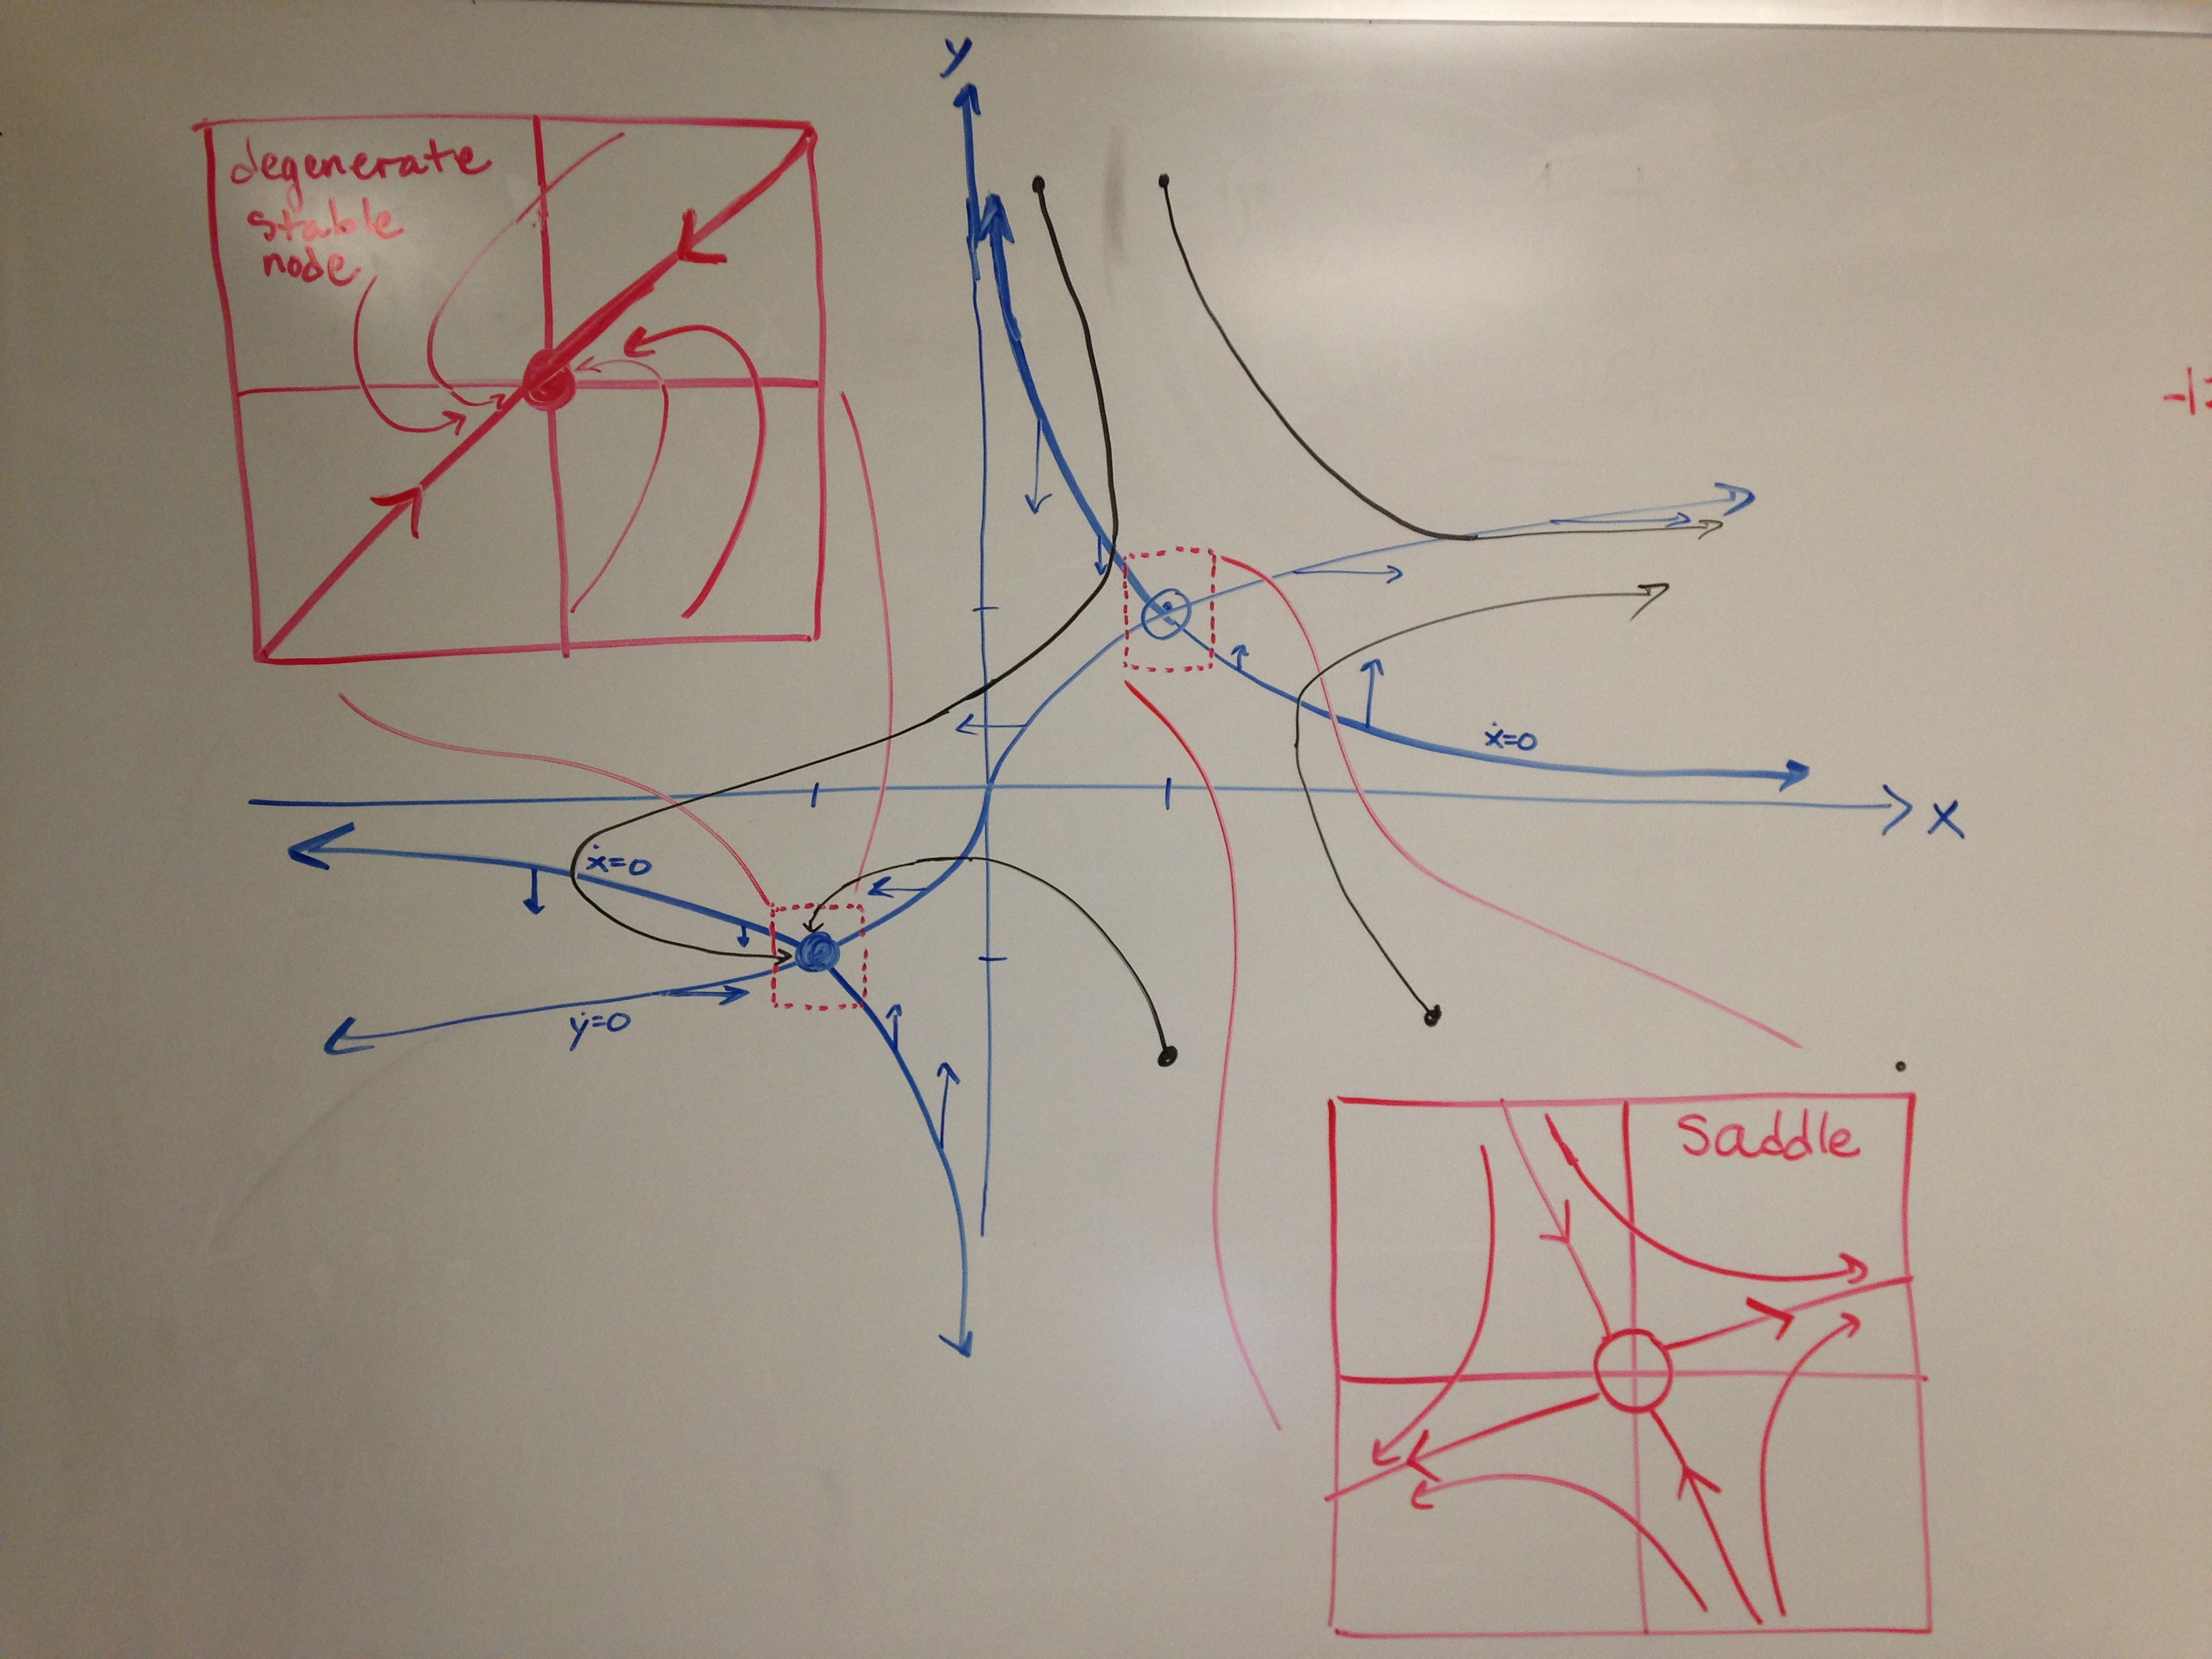
\includegraphics[width=400px]{figures/3_drawing.jpg}
    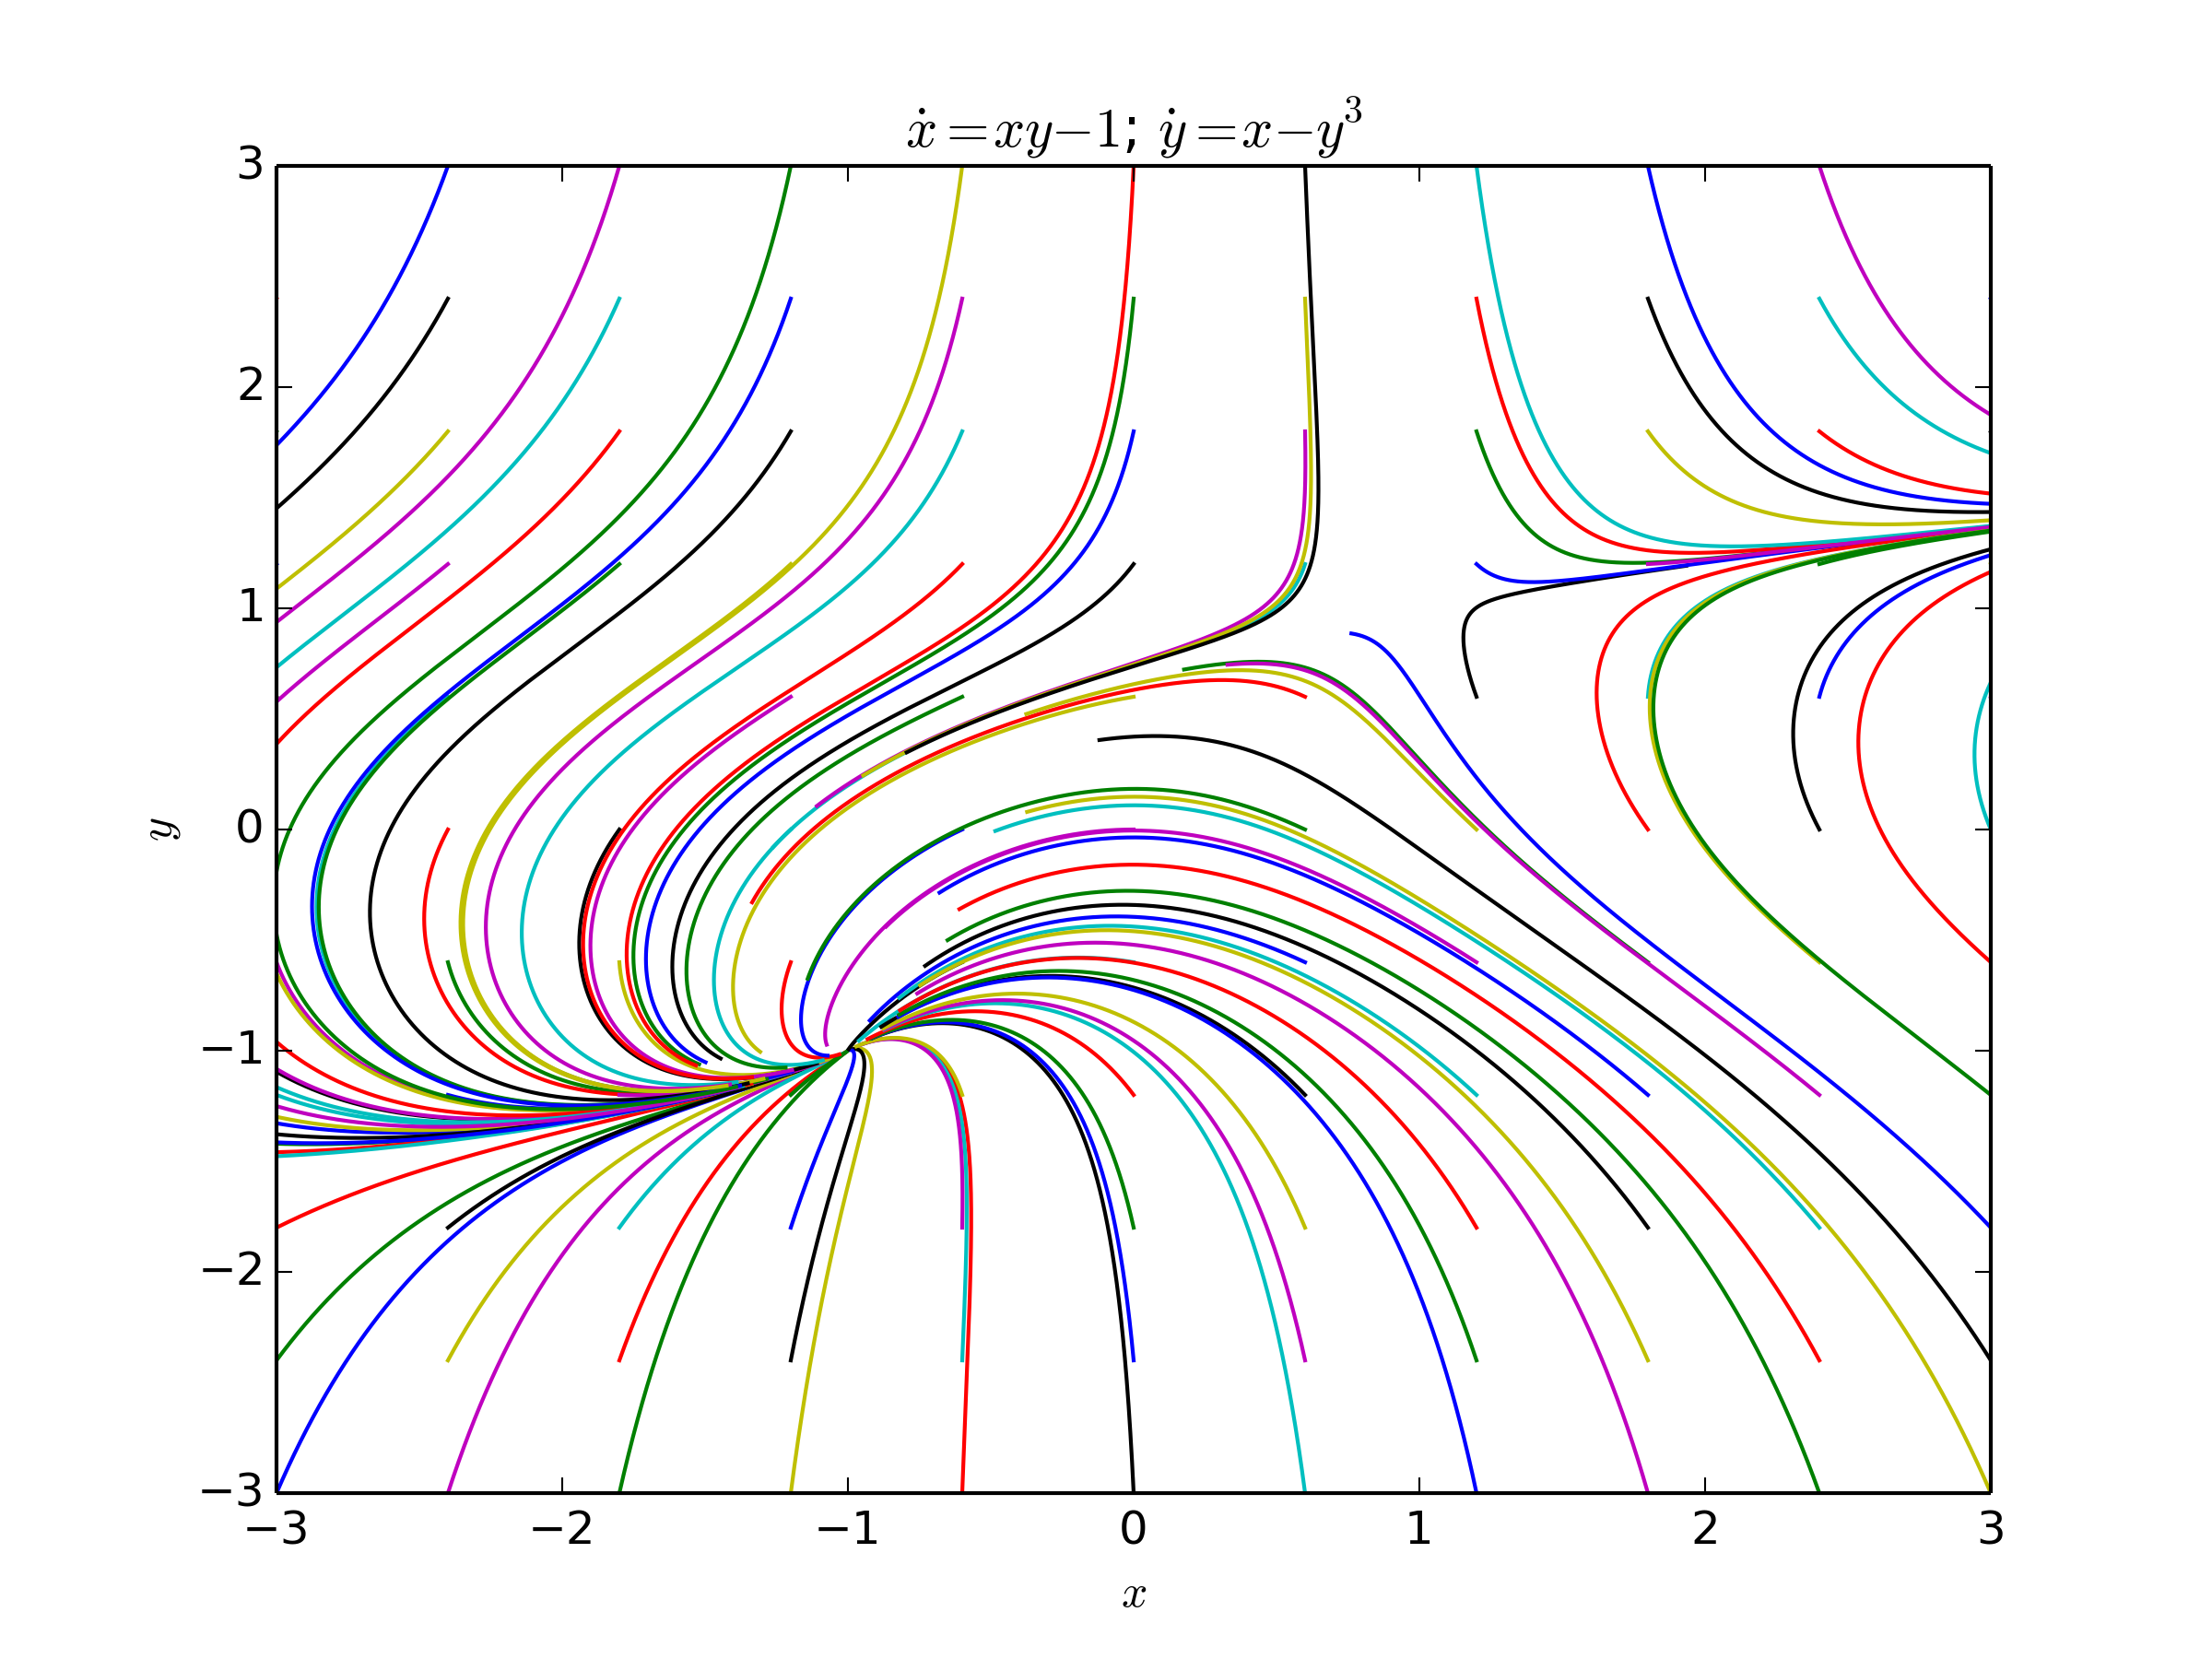
\includegraphics[width=400px]{figures/3_simulation.png}
\end{figure}

\FloatBarrier
\section*{Problem 4}
\emph{Problem 6.4.1}

\subsection*{ a)}
\emph{The following is a ``rabbits vs. sheep'' model of two species competing for resources (in this case, rabbits and sheep competing for grass).  They are discussed in \S6.4 in the book.}
\begin{align*}
	\dot{x} &= x(3 - x - y) \\
	\dot{y} &= y(2 - x - y)
\end{align*}
\emph{Find the fixed points, investigate their stability and draw plausible phase portraits.} \\

$\dot{x} = 0 \implies x = 0$ or $y = -x + 3$.  $\dot{y} = 0 \implies y = 0$ or $y = -x + 2$.  Thus the fixed points are
\begin{align*}
	\vec{x_A}^* = \qty(\begin{array}{c}0 \\ 0\end{array})\ \ \ \vec{x_B}^* = \qty(\begin{array}{c}3 \\ 0\end{array})\ \ \ \vec{x_C}^* = \qty(\begin{array}{c}0 \\ 2\end{array})
\end{align*}
The Jacobian is
\begin{align*}
	J &= \qty(\begin{array}{cc}
		3 - 2x - y & -x \\
		-y & 2 - x - 2y
	\end{array}) \\
	\implies J_{\vec{x_A}^*} &= \qty(\begin{array}{cc}
		3 & 0 \\
		0 & 2
	\end{array})\ \ \text{and}\ \ J_{\vec{x_B}^*} = \qty(\begin{array}{cc}
		-3 & -3 \\
		0 & -1
	\end{array})\ \ \text{and}\ \ J_{\vec{x_C}^*} = \qty(\begin{array}{cc}
		1 & 0 \\
		-2 & -2
	\end{array})
\end{align*}
Thus the eigenvalues for $\vec{x_A}^*$ are $3$ and $2$, and so it is an unstable node.  The eigenvalues for $\vec{x_B}^*$ are $-3$ and $-1$, and so it is a stable node.  The eigenvalues for $\vec{x_C}^*$ are $1$ and $-2$, and so it is a saddle.

\subsection*{ b)}
\emph{Check your answers by generating a phase portrait with Matlab.  (Simulate several initial conditions, and plot $x$ and $y$)}

\begin{figure}[ht]
    \centering
    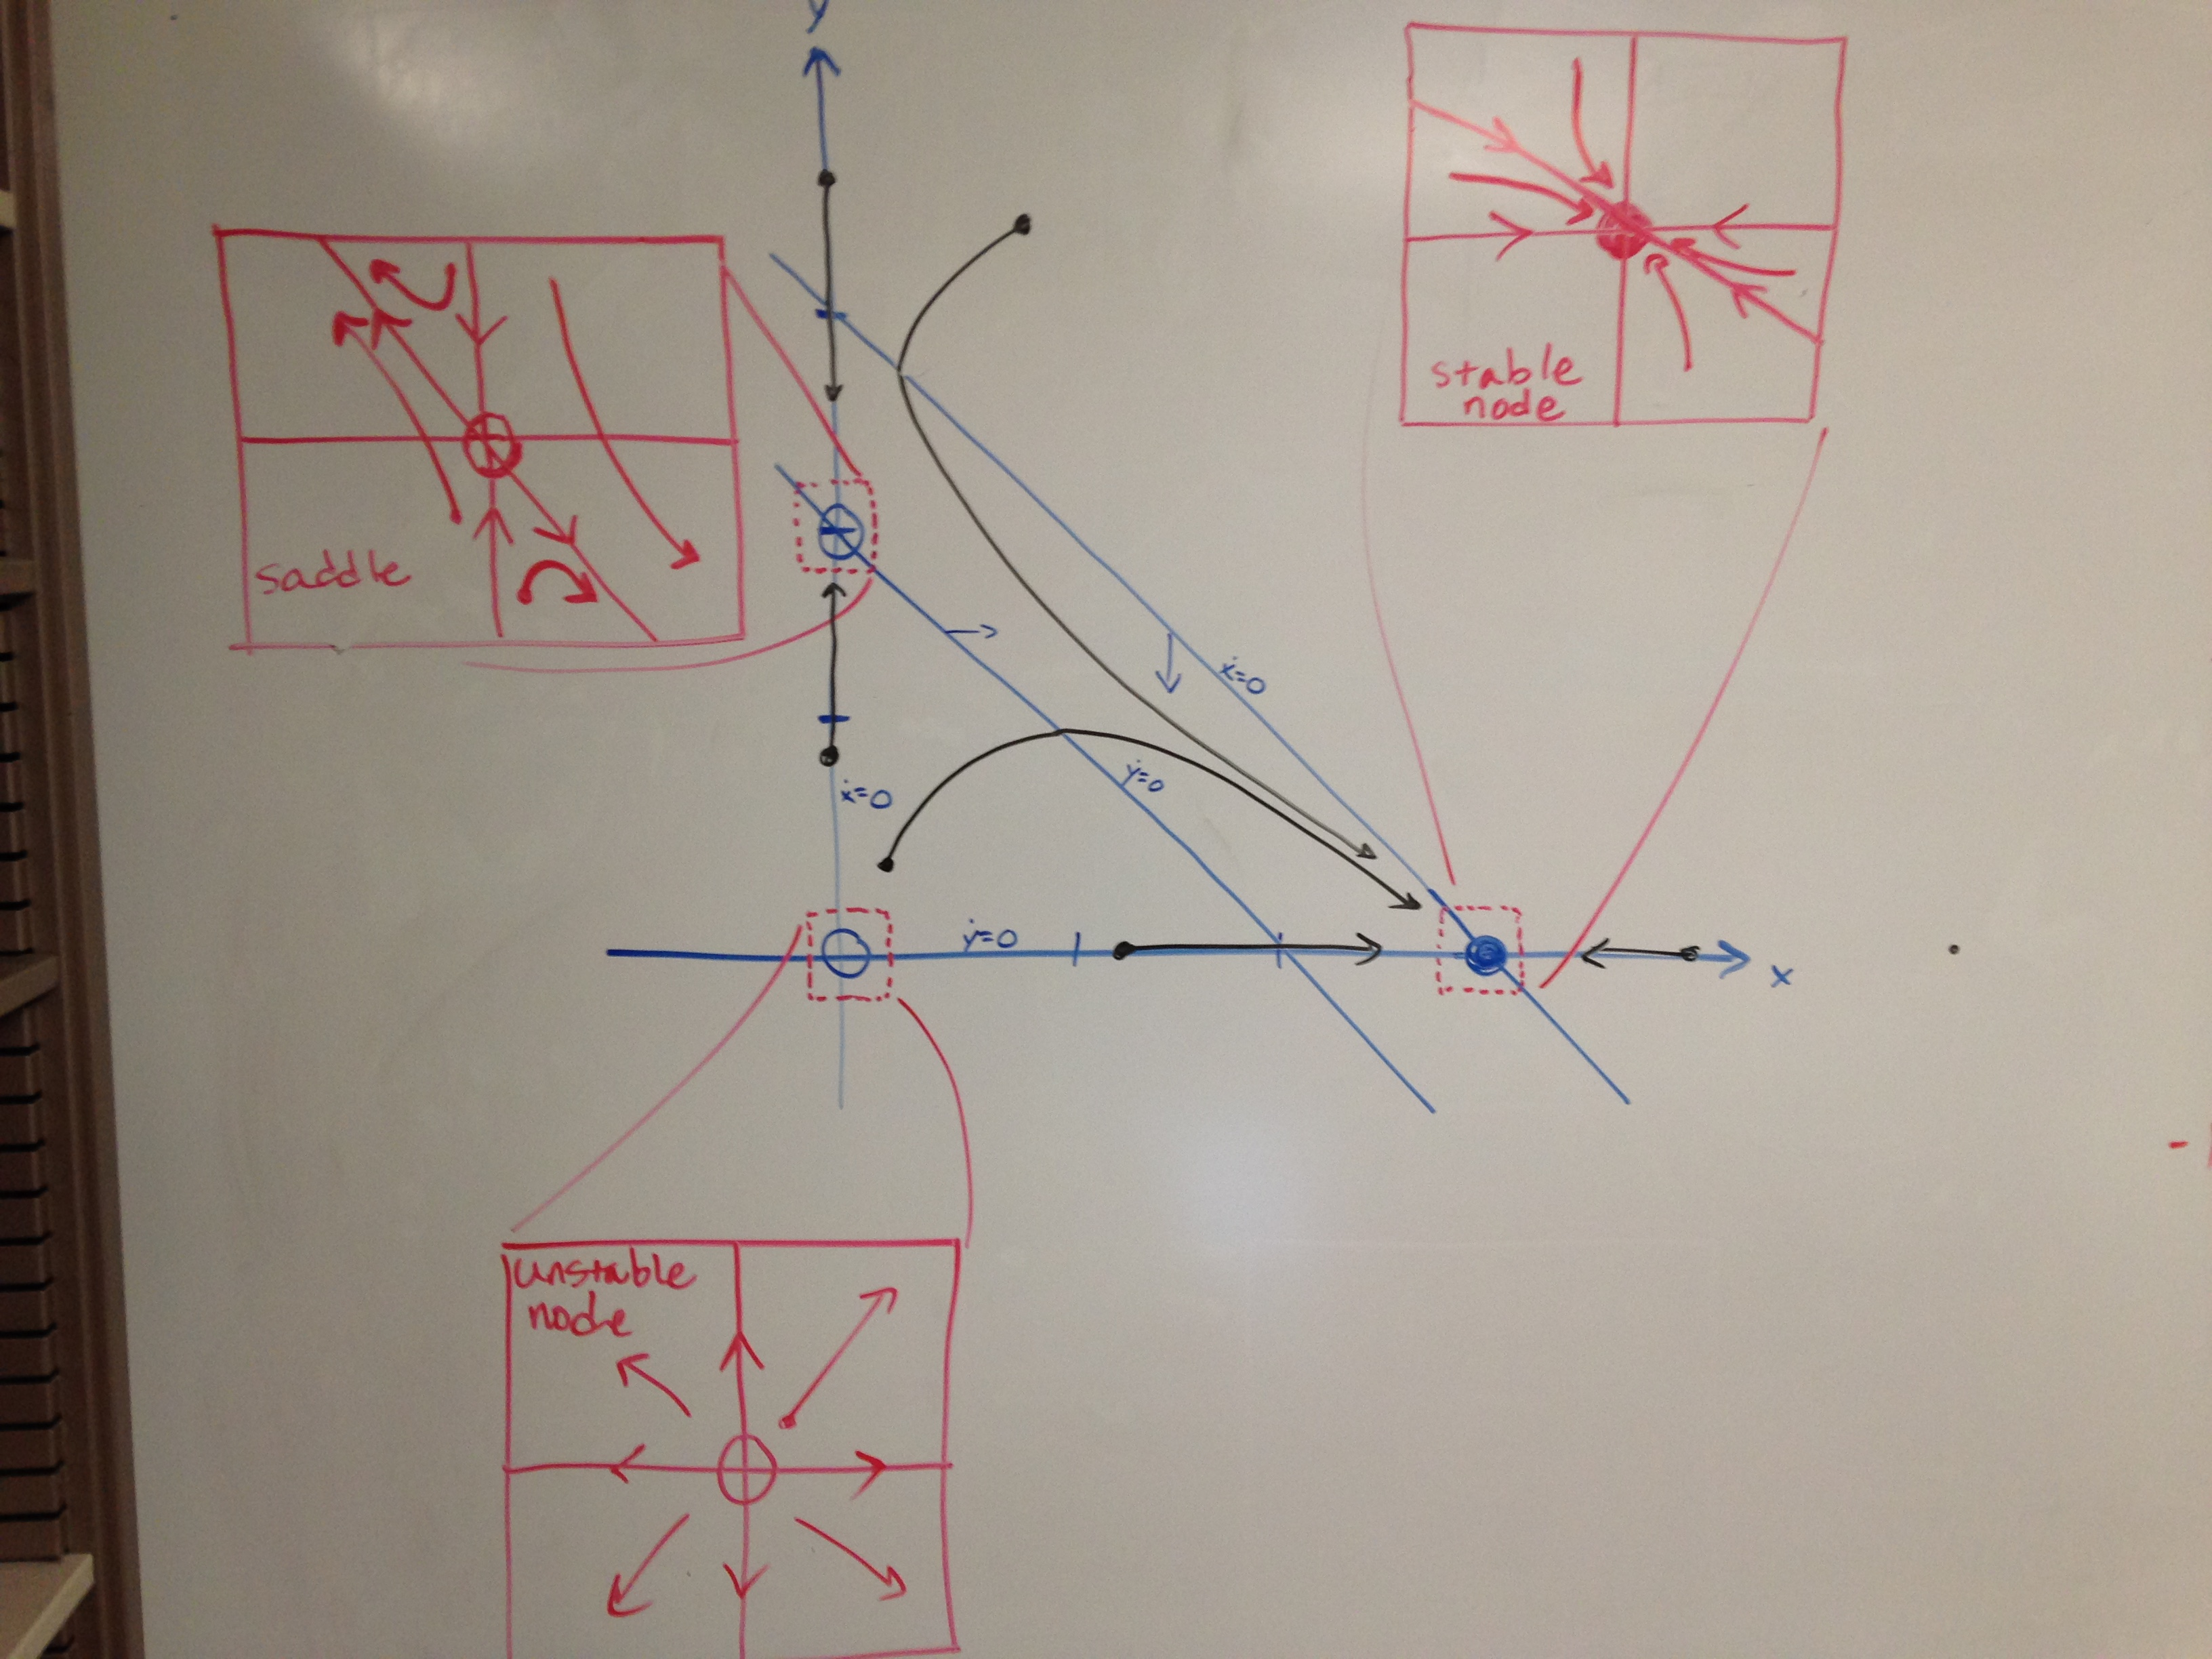
\includegraphics[width=400px]{figures/4_drawing.jpg}
    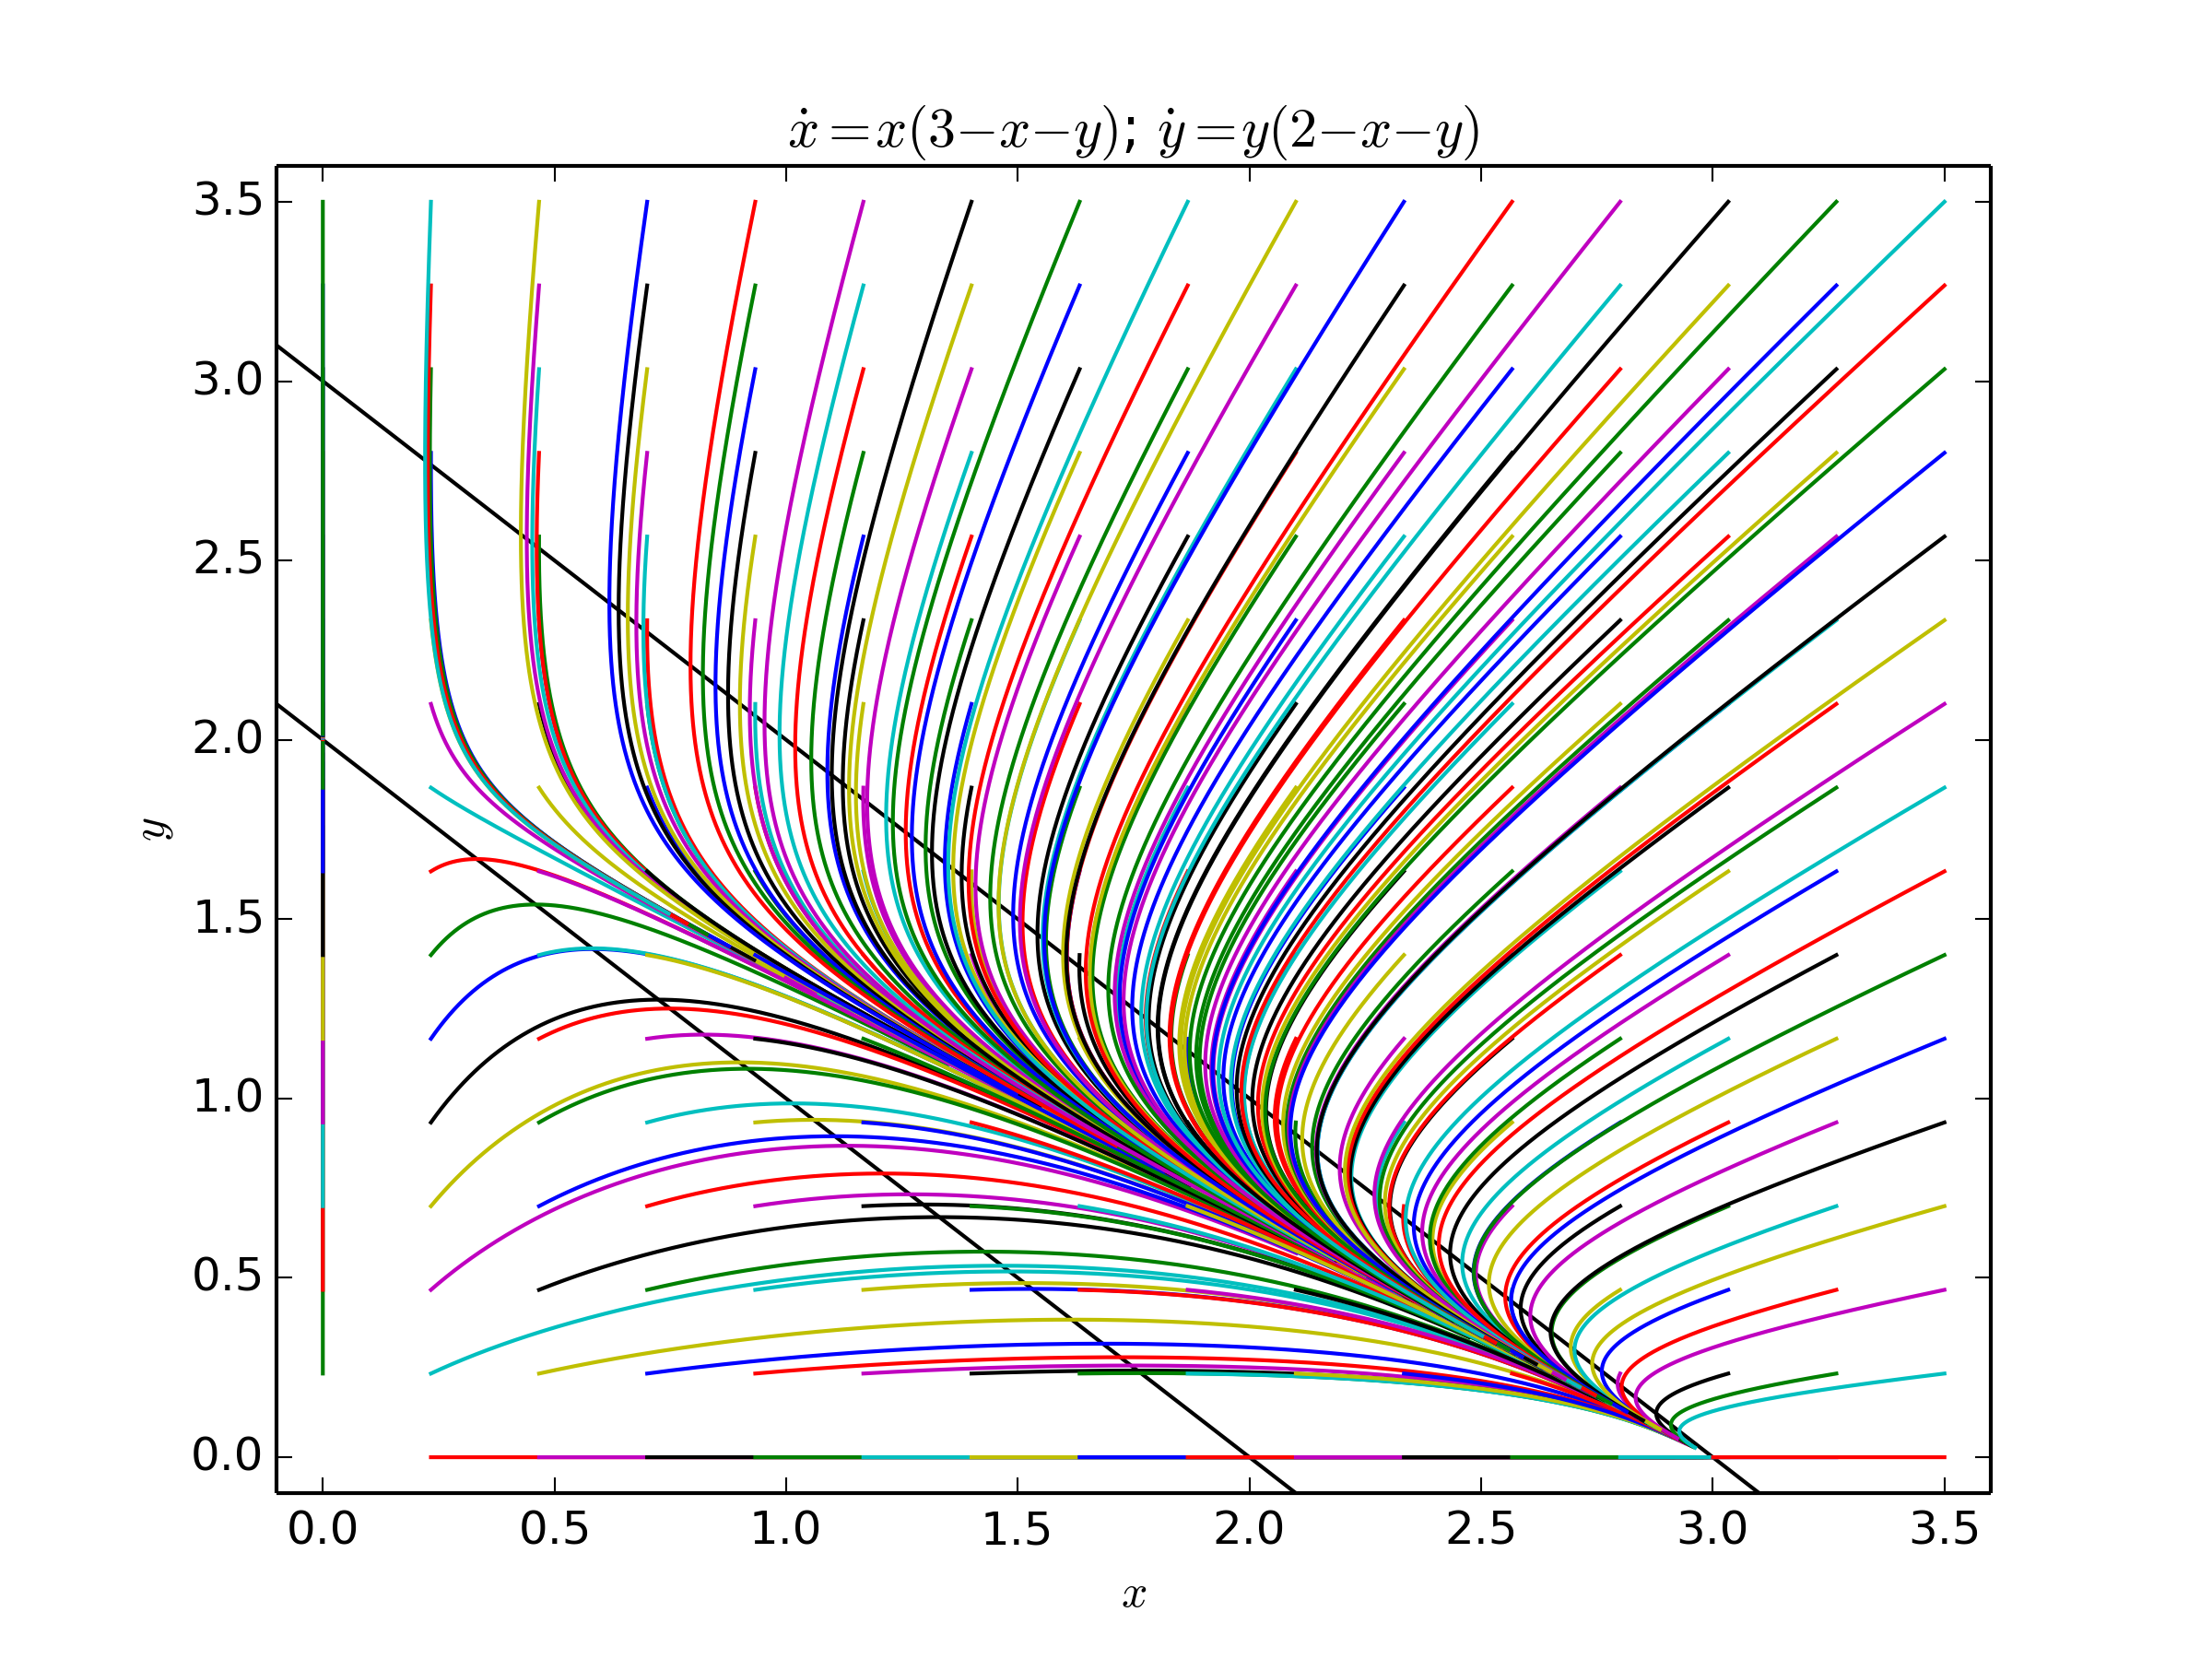
\includegraphics[width=400px]{figures/4_simulation.png}
\end{figure}

\end{document}
